\documentclass[11pt]{article}
\usepackage{../mystyle}

% Each solution stays on one page (invisible, unbreakable box).
% Solutions taller than a page use \begin{solbox}[long]: new page, then breakable.
\tcbset{long/.style={breakable, before={\clearpage}}}
\newtcolorbox{solbox}[1][]{blanker, before skip=4pt, after skip=10pt, #1}

\title{FIT1058 --- Course Notes Exercises \& Solutions\\
\large CN end-of-chapter exercises (boxed) with solutions where done}
\author{Alston}
\date{Semester 2, 2026}

\begin{document}
\maketitle
\tableofcontents

\newpage
\section{Chapter 1: Sets}
% CN 1.16 Exercises (p.28--35)

% ======================================================================
\begin{exercise}{1}
    Why does the set difference only satisfy (1.9) $\bigl(|B\setminus A| = |B|-|A|\bigr)$
    when $A\subseteq B$? How would you modify (1.9) so that it covers any set
    difference $B\setminus A$? What extra information about the sets would you
    need, in order to determine $|B\setminus A|$?
\end{exercise}

% ======================================================================
\begin{exercise}{2}
    In C, \texttt{int monthNumber;} declares a variable of type \texttt{int},
    and \texttt{char monthName[10];} declares a string of at most 9 characters.
    Let \texttt{Int} be the set of possible values for a variable of type
    \texttt{int}, and \texttt{String} the set of possible values for a string of
    at most 9 letters.
    \begin{enumerate}[label=(\alph*)]
        \item The statement
\begin{verbatim}
struct aNewType {
    int year;
    char monthName[10];
} monthBothWays;
\end{verbatim}
        creates a type for objects consisting of any int followed by any string.
        Using \texttt{Int}, \texttt{String} and a standard set operation, what
        set is represented by \texttt{aNewType}?
        \item The statement
\begin{verbatim}
union anotherNewType {
    int year;
    char monthName[10];
} monthEitherWay;
\end{verbatim}
        creates a type for objects that can be either an int or a string (only
        one at a time). What set is represented by \texttt{anotherNewType}?
    \end{enumerate}
\end{exercise}

% ======================================================================
\begin{exercise}{3}
    Suppose $A$ and $B$ are subsets of some universal set $U$.
    \begin{enumerate}[label=(\alph*)]
        \item If $A\subseteq B$, what is $A\cup B$?
        \item If $A\not\subseteq B$, what can you say about $A\cup B$?
        \item Complete the following: $A\subseteq B$ if and only if
              $A\cup B = \underline{\hspace{2cm}}$.
        \item Devise another equivalent condition for $A\subseteq B$ involving
              intersection instead of union.
        \item Devise another equivalent condition for $A\subseteq B$ involving
              set difference.
    \end{enumerate}
\end{exercise}

% ======================================================================
\begin{exercise}{4}
    Consider diagrams of the following type (e.g.\ for $\{a,b\}$: $\emptyset$ at
    the bottom, $\{a\},\{b\}$ in the middle, $\{a,b\}$ at the top). The
    requirements are:
    \begin{itemize}
        \item Sets are written in their usual textual form (not Venn diagrams).
        \item Smaller sets are lower on the page than larger sets; sets of the
              same size are on the same horizontal level.
        \item If $X\subset Y$ and $|Y|=|X|+1$ then there is an arrow from $X$ to $Y$.
        \item The diagram is as neat and symmetric as possible.
    \end{itemize}
    \begin{enumerate}[label=(\alph*)]
        \item Draw a diagram of this type that shows all subsets of $\{a,b,c\}$
              and the subset relation among them.
        \item For every pair $X,Y$ with $X\subset Y$ and $|Y|=|X|+1$, label the
              corresponding arrow by the sole member of $Y\setminus X$.
        \item If you could draw in three dimensions, how could you draw this
              diagram in a natural way?
        \item For a set of $n$ elements, how many sets and how many arrows does a
              diagram of this type have?
        \item For each element of the $n$-element set in (d), how many arrows are
              labelled by that element?
        \item Suppose $X\subseteq Y$. How many directed paths (along arrows,
              forwards only) are there from $X$ to $Y$? Give an expression.
        \item With $X,Y$ as in (f), what is the maximum number of mutually
              internally disjoint paths from $X$ to $Y$? (Two paths are
              internally disjoint if no internal set on either path appears
              anywhere on the other path.)
        \item Explain how to use the diagram to find, for any two sets in it,
              their union and intersection.
    \end{enumerate}
\end{exercise}

% ======================================================================
\begin{exercise}{5}
    Given $U=\{e_1,e_2,\dots,e_n\}$, the \emph{characteristic string} of a subset
    $A\subseteq U$ is the $n$-bit string $b_1b_2\cdots b_n$ where
    \[
        b_i = \begin{cases} 1, & e_i\in A;\\ 0, & e_i\notin A.\end{cases}
    \]
    Write down the characteristic string of each of the subsets of a set of three
    elements. List them, one above the other, so that each differs from the one
    above it in just one bit. See if you can extend this to subsets of a set of
    $n$ elements.
\end{exercise}

% ======================================================================
\begin{exercise}{6}
    Two intersecting sets $A,B$ divide the plane into four basic regions:
    $\overline{A\cup B}$, $A\cap B$, $A\setminus B$, $B\setminus A$. Three sets
    can divide the plane into eight regions.
    \begin{enumerate}[label=(\alph*)]
        \item Label each basic region of a Venn diagram for three sets $A,B,C$
              with appropriate intersections of sets.
    \end{enumerate}
    A \emph{general Venn diagram} for $n$ sets $A_1,\dots,A_n$ is one in which
    every intersection of the form
    \[
        (A_1 \text{ or } \overline{A_1})\cap(A_2\text{ or }\overline{A_2})\cap\cdots
        \cap(A_n\text{ or }\overline{A_n})
    \]
    corresponds to one of the basic regions, so there are $2^n$ basic regions.
    \begin{enumerate}[label=(\alph*),start=2]
        \item What is the maximum number of sets for which a general Venn diagram
              can be drawn in which all the sets are circles of the same size?
        \item Draw a general Venn diagram in the plane for four sets. You can use
              closed curves other than circles.
        \item How could you draw a three-dimensional general Venn diagram using
              four sets, each represented as a sphere?
    \end{enumerate}
\end{exercise}

% ======================================================================
\begin{exercise}{7}
    Prove that if $A\subseteq B$ then $\power{A}\subseteq\power{B}$.
\end{exercise}

% ======================================================================
\begin{exercise}{8}
    Consider the sequence of binomial coefficients
    $\binom n0,\binom n1,\binom n2,\dots,\binom n{n-1},\binom nn$.
    \begin{enumerate}[label=(\alph*)]
        \item Using one of the formulas for $\binom nr$, prove that these
              binomial coefficients increase as $r$ goes from $0$ to
              $\lfloor n/2\rfloor$ and then decrease as $r$ goes from
              $\lceil n/2\rceil$ to $n$. (In the odd case, what happens when $r$
              goes from $(n-1)/2$ to $(n+1)/2$?)
        \item Prove that, for every integer $r$ with $1\le r\le n-1$,
              \[
                  \binom nr^2 > \binom n{r-1}\binom n{r+1}.
              \]
              (The sequence is \emph{strictly log-concave}.)
        \item You choose an ordered pair of subsets of size $r$ of a set of size
              $n$ (no other restriction). Your friend chooses one subset of size
              $r-1$ and another of size $r+1$. Who has more options? Does the
              answer depend on $n$ and $r$? Is there any situation where the
              numbers of choices are the same?
    \end{enumerate}
\end{exercise}

% ======================================================================
\begin{exercise}{9}
    Express $|A\cup B|$ in terms of $|A|,|B|,|A\cap B|$.
\end{exercise}

\begin{exercise}{10}
    Express $|A\cap B|$ in terms of $|A|,|B|,|A\cup B|$.
\end{exercise}

\begin{exercise}{11}
    Express $|A\cup B\cup C|$ in terms of
    $|A|,|B|,|C|,|A\cap B|,|A\cap C|,|B\cap C|,|A\cap B\cap C|$.
\end{exercise}

\begin{exercise}{12}
    Express $|A\cap B\cap C|$ in terms of
    $|A|,|B|,|C|,|A\cup B|,|A\cup C|,|B\cup C|,|A\cup B\cup C|$.
\end{exercise}

% ======================================================================
\begin{exercise}{13}
    Suppose we have sets $A_1,\dots,A_n$. For each $k$, let
    \[
        i_k := \text{sum of all sizes of intersections of $k$ of the sets.}
    \]
    E.g.\ for $n=3$: $i_1=|A_1|+|A_2|+|A_3|$,
    $i_2=|A_1\cap A_2|+|A_1\cap A_3|+|A_2\cap A_3|$, $i_3=|A_1\cap A_2\cap A_3|$.

    Rewrite your expressions for $|A\cup B|$ and $|A\cup B\cup C|$ in terms of
    $i_1,i_2,\dots$. Then write out a general expression for
    $|A_1\cup\cdots\cup A_n|$. Pay careful attention to the sign of the last term.
\end{exercise}

% ======================================================================
\begin{exercise}{14}
    Now let
    \[
        u_k := \text{sum of all sizes of unions of $k$ of the sets.}
    \]
    Rewrite your expressions for $|A\cap B|$ and $|A\cap B\cap C|$ in terms of
    $u_1,u_2,\dots$. Then write out a general expression for
    $|A_1\cap\cdots\cap A_n|$. Pay careful attention to the sign of the last term.
\end{exercise}

% ======================================================================
\begin{exercise}{15}
    Express $|A\triangle B|$ in terms of the sizes of some other sets in three
    different ways.
\end{exercise}

\begin{exercise}{16}
    Draw a Venn diagram for general sets $A,B,C$ and shade the region(s) that
    form $A\triangle B\triangle C$.
\end{exercise}

\begin{exercise}{17}
    Prove that, for any sets $A$ and $B$,
    \[
        (A\cup B)\triangle(A\cap B) = A\triangle B.
    \]
\end{exercise}

\begin{exercise}{18}
    Suppose $A_1,\dots,A_n$ are sets. How would you characterise
    $A_1\triangle A_2\triangle\cdots\triangle A_n$? More specifically, its members
    are those that satisfy some condition on how many of the sets they belong to.
    What is that condition?
\end{exercise}

% ======================================================================
\begin{exercise}{19}
    If $A$ and $B$ are sets, does $\overline{A\times B}$ equal
    $\overline A\times\overline B$? If so, prove it. If not: give an example when
    it does not hold; characterise those cases when it does hold; and determine
    what can be said about the relationship between them.
\end{exercise}

\begin{exercise}{20}
    Write down all partitions of $\{1,2,3,4\}$ into three parts.
\end{exercise}

\begin{exercise}{21}
    Suppose $A,B,C\subseteq U$ are nonempty sets such that all basic regions in
    their general Venn diagram are nonempty (see Exercise 6). Then $A,B,C$ define
    a partition of $U$ into eight parts. What are those parts? Express each part
    in terms of one or more of $A,B,C$ using set operations.
\end{exercise}

\begin{exercise}{22}
    Does $\R$ have a partition in which all parts are
    \begin{enumerate}[label=(\alph*)]
        \item open intervals?
        \item half-open half-closed intervals?
        \item closed intervals?
    \end{enumerate}
\end{exercise}


\newpage
\section{Chapter 2: Functions}
% CN 2.19 Exercises (p.76--84)

% ======================================================================
\begin{exercise}{1}
    Let $A$ be a finite set. How many indicator functions with domain $A$ are
    there?
\end{exercise}
\begin{solbox}
\begin{solution}
    An indicator function is defined by
    \[
        \chi_A(x) = \begin{cases} 1 & \text{if } x\in A \\
            0 & \text{if } x\notin A \end{cases}
    \]

    Let $|A|=n$. The number of functions $\chi: A\to\{0,1\}$ equals
    the number of ways to independently assign each of the $n$
    elements of $A$ a value in $\{0,1\}$, which is $2^n$.

    Equivalently, each such function corresponds to exactly one
    subset $X\subseteq A$ (namely $X=\{x\in A : \chi(x)=1\}$), so the
    number of indicator functions equals $|\mathcal P(A)| = 2^n$.
\end{solution}
\end{solbox}

\begin{exercise}{2}
    Let $A$ and $B$ be any sets. Express the indicator functions of each of the
    following in terms of $\chi_A$ and $\chi_B$.
    \begin{enumerate}[label=(\alph*)]
        \item $\overline A$
        \item $A\cap B$
        \item $A\setminus B$
        \item $A\triangle B$
    \end{enumerate}
\end{exercise}
\begin{solbox}
\begin{solution}
    \textbf{(a)}
    \[
        \chi_{\overline A}(x) = 1-\chi_A(x).
    \]

    \textbf{(b)} $x\in A\cap B \iff x\in A \wedge x\in B$, so
    \[
        \chi_{A\cap B} = \chi_A\cdot\chi_B.
    \]

    \textbf{(c)} $x\in A\setminus B \iff x\in A \wedge x\notin B$, so
    \[
        \chi_{A\setminus B} = \chi_A\cdot\chi_{\overline B}
        = \chi_A\cdot(1-\chi_B) = \chi_A - \chi_A\chi_B.
    \]

    \textbf{(d)} Since $A\triangle B = (A\setminus B)\cup(B\setminus
    A)$ is a disjoint union,
    \[
        \chi_{A\triangle B} = \chi_{A\setminus B}+\chi_{B\setminus A}
        = (\chi_A-\chi_A\chi_B)+(\chi_B-\chi_A\chi_B)
        = \chi_A+\chi_B-2\chi_A\chi_B.
    \]
\end{solution}
\end{solbox}

\begin{exercise}{3}
    If $f:A\to\R$ and $g:A\to\R$, their sum $f+g:A\to\R$ is defined by
    $(f+g)(x)=f(x)+g(x)$. What is the sum of all the indicator functions of all
    the subsets of a finite set?
\end{exercise}
\begin{solbox}
\begin{proof}
    Let $A$ be a finite set with $|A|=n$. Since function addition is
    defined pointwise, for any $x_i\in A$,
    \[
        \left(\sum_{X\subseteq A}\chi_X\right)(x_i)
        = \sum_{X\subseteq A}\chi_X(x_i).
    \]

    Since $\chi_X(x_i)=1$ if $x_i\in X$ and $0$ otherwise, this sum
    counts the number of subsets $X\subseteq A$ containing $x_i$.

    \textbf{Method 1 (direct count).} A subset containing $x_i$ is
    formed by fixing $x_i$ to be included, and choosing freely,
    independently, whether each of the remaining $n-1$ elements is
    included. This gives $2^{n-1}$ such subsets.

    \textbf{Method 2 (summing over subset sizes).} For each size
    $k=1,\dots,n$, the number of size-$k$ subsets containing $x_i$ is
    obtained by fixing $x_i$ as one member and choosing the
    remaining $k-1$ members from the other $n-1$ elements:
    $\binom{n-1}{k-1}$. Summing over all sizes,
    \[
        \sum_{X\subseteq A}\chi_X(x_i)
        = \sum_{k=1}^{n}\binom{n-1}{k-1}
        = \sum_{j=0}^{n-1}\binom{n-1}{j} = 2^{n-1},
    \]
    using the binomial identity $\sum_{j=0}^{m}\binom{m}{j}=2^m$
    with $m=n-1$.

    Both methods agree: $\left(\sum_{X\subseteq A}\chi_X\right)(x_i)
    = 2^{n-1}$ for every $x_i\in A$, independent of which $x_i$ is
    chosen. So $\sum_{X\subseteq A}\chi_X$ is the constant function
    on $A$ with value $2^{n-1}$.
\end{proof}
\end{solbox}

\begin{exercise}{4}
    Draw a Venn diagram showing each of the following sets of functions and the
    relationships between them: functions, injections, surjections, bijections,
    identity functions, binary relations, ternary relations, relations.
\end{exercise}

% ======================================================================
\begin{exercise}{5}
    Functions can be viewed as sets of ordered pairs, so we can combine them
    using set operations. Suppose $f:A\to B$ and $g:C\to D$ are functions. Which
    of the following is always a function?
    \[
        f\cap g;\quad f\cup g;\quad f\setminus g;\quad g\setminus f;\quad
        f\triangle g;\quad f\times g.
    \]
    For each that is always a function, give its definition in the usual form
    (domain, codomain, rule in terms of $f$ and $g$). For each that is not
    necessarily a function, explain why (e.g.\ with examples).
\end{exercise}
\begin{solbox}
\begin{proof}
    Recall that $R\subseteq A\times B$ is a function if and only if
    $R$ satisfies both:
    \begin{itemize}
        \item \textbf{Existence}: $\{x\in A : (x,y)\in R \text{ for
            some } y\in B\} = A$;
        \item \textbf{Uniqueness (well-definedness)}: for every
            $x\in A$, the set $R(x)=\{y\in B : xRy\}$ contains
            exactly one element.
    \end{itemize}

    \medskip
    \textbf{(i) $f\cap g$.}
    \[
        (f\cap g)(x) = \{f(x)\}\cap\{g(x)\}.
    \]
    When $f(x)=g(x)$: $(f\cap g)(x) = \{f(x)\}$.
    When $f(x)\ne g(x)$: $(f\cap g)(x) = \emptyset$ --- does not
    exist. So $f\cap g$ is \emph{not necessarily} a function; it can
    fail \textbf{existence}.

    \medskip
    \textbf{(ii) $f\cup g$.} \label{5ii}
    \[
        (f\cup g)(x) = \{f(x)\}\cup\{g(x)\}.
    \]
    When $f(x)=g(x)$: $|(f\cup g)(x)|=1$.
    When $f(x)\ne g(x)$: $|(f\cup g)(x)|=2$. So $f\cup g$ is
    \emph{not necessarily} a function; it can fail
    \textbf{uniqueness}.

    \medskip
    \textbf{(iii) $f\setminus g$.}
    \[
        (f\setminus g)(x) = \{f(x)\}\setminus\{g(x)\}.
    \]
    When $f(x)=g(x)$: $|f\setminus g|=0$ --- does not exist.
    When $f(x)\ne g(x)$: $|f\setminus g|=1$. So $f\setminus g$ is
    \emph{not necessarily} a function; it can fail
    \textbf{existence}.

    \medskip
    \textbf{(iv) $g\setminus f$.}
    By the same argument as (iii) with the roles of $f,g$
    interchanged, $g\setminus f$ is \emph{not necessarily} a
    function.

    \medskip
    \textbf{(v) $f\triangle g$.}
    \[
        (f\triangle g)(x) = \{(f\setminus g)(x)\}
        \cup \{(g\setminus f)(x)\}.
    \]
    When $f(x)=g(x)$: $|f\triangle g|=0$ --- does not exist.
    When $f(x)\ne g(x)$: $|f\triangle g|=2$. So $f\triangle g$ is
    \emph{not necessarily} a function; depending on $f,g$, it can
    fail either \textbf{existence} or \textbf{uniqueness}.

    \medskip
    \textbf{(vi) $f\times g$.}
    \[
        f\times g = \{((a,b),(c,d)) : (a,b)\in f,\ (c,d)\in g\}.
    \]
    This defines a function
    \[
        f\times g : A\times C \to B\times D, \qquad
        (f\times g)(x,y) = (f(x), g(y)).
    \]
    \textbf{Existence}: for all $(x,y)\in A\times C$, since $f$ and
    $g$ are functions, $f(x)$ and $g(y)$ must exist, so
    $(f(x),g(y))$ exists.
    \textbf{Uniqueness}: since $f(x)$ and $g(y)$ are each unique,
    the pair $(f(x),g(y))$ is unique.
    So $f\times g$ is \emph{always} a function.
\end{proof}
\end{solbox}

\begin{exercise}{6}
    Suppose $f:A\to B$ and $g:C\to D$ are functions with disjoint domains,
    $A\cap C=\emptyset$. Is the disjoint union $f\sqcup g$ always a function? If
    so, give its definition in terms of $f$ and $g$. If not, why not?
\end{exercise}
\begin{solbox}
\begin{solution}
    By \hyperref[5ii]{5(ii)} $f \cup g $ is always a function.
\end{solution}
\end{solbox}

\begin{exercise}{7}
    Give an example of a function $f:\N\times\N\to\N$ which is an injection.
    Even better, give one which is a bijection.
\end{exercise}

% ======================================================================
\begin{exercise}{8}
    A \emph{bitstring} is a member of $\{0,1\}^*$.
    \begin{enumerate}[label=(\alph*)]
        \item Give a bijection from $\{0,1\}^*$ to $\N$.
    \end{enumerate}
    Let $\{0,1\}^{*+}$ denote the set of all finite nonempty tuples of
    bitstrings, e.g.\ $(011,1,10001)$, $(10,10,10,10)$, $(\epsilon,1011)$,
    $(1010010001)$.
    \begin{enumerate}[label=(\alph*),start=2]
        \item (Challenge) Give a bijection from $\{0,1\}^{*+}$ to $\{0,1\}^*$.
    \end{enumerate}
\end{exercise}
\begin{solbox}[long]
\begin{solution}[(a)]

\paragraph{Setup: grouping by length.} For each $n\ge0$, there are $2^n$
bitstrings of length $n$. We assign each bitstring a natural number
(``index'') as follows:

\begin{center}
\begin{tabular}{c c c c}
\hline
length & bitstring & number of bitstrings & index $\in \N$ \\
\hline
$0$ & $\varepsilon$ & $1$ & $0$ \\
$1$ & $0,1$ & $2=2^1$ & $1,2$ \\
$2$ & $00,01,10,11$ & $2^2$ & $3,4,5,6$ \\
$\vdots$ & $\vdots$ & $\vdots$ & $\vdots$ \\
$n$ & $\cdots$ & $2^n$ & $\cdots$ \\
\hline
\end{tabular}
\end{center}

\paragraph{Defining $f_n$.} For $\{0,1\}^n$, the value of a string is a
member of $\{0,1,\dots,2^n-1\}$. Define $f_n$ to be the value of
$\{0,1\}^n$:
\[
    f_n : \{0,1\}^n \longrightarrow \{0,1,\dots,2^n-1\}, \qquad
    f_n(s) = f_n(s_1 s_2 \cdots s_n) = \sum_{i=1}^n s_i\cdot 2^{n-i}.
\]

\begin{claim}
    For every $n$, $f_n$ is a bijection.
\end{claim}
\begin{proof}
    When $n=0$: $f_0:\{\varepsilon\}\to\{0\}$, $f_0(\varepsilon)=0$, is a
    bijection.

    Assume $f_{n-1}:\{0,1\}^{n-1}\to\{0,\dots,2^{n-1}-1\}$ is a bijection.

    For $f_n$,
    \[
        f_n(s_1\cdots s_n) = s_1\cdot 2^{n-1} + \sum_{i=2}^n s_i\cdot 2^{n-i}
        = s_1\cdot 2^{n-1} + f_{n-1}(s_2\cdots s_n).
    \]

    When $s_1=0$: $f_n(s_1\cdots s_n)\in\{0,\dots,2^{n-1}-1\}$.

    When $s_1=1$: $f_n(s_1\cdots s_n) \in \{2^{n-1},\dots,2^{n-1}-1+2^{n-1}\}
    = \{2^{n-1},\dots,2^n-1\}$.

    We know that $f_n(s_1\cdots s_n)\in\{0,\dots,2^n-1\}$.

    By induction, we know that $f_n$ is a bijection.
\end{proof}

\paragraph{Starting index of each length group.} Observe that, for
length $=n$, the starting index is equal to the number of bitstrings of
length $=0$ to length $=n-1$:
\[
    \text{starting index} = \sum_{k=0}^{n-1} |\{0,1\}^k| = \sum_{k=0}^{n-1} 2^k
    = \frac{2^n-1}{2-1} = 2^n-1.
\]

So, $f : \{0,1\}^* \to \N$ is equal to $(2^n-1) + $ (position of bitstring
in the group of the length):
\[
    f(s) = (2^n-1) + f_n(s), \qquad n = |s|.
\]

\begin{claim}
    $f$ is a bijection.
\end{claim}
\begin{proof}
    We know $f(s) \in \big[\,2^{|s|}-1,\ 2^{|s|+1}-2\,\big]$.

    \textbf{First, we prove $f$ is injective.}

    \emph{Case 1: $s\ne t$ and $|s|\ne|t|$.} Let $|s|<|t|$. Then
    \[
        f(s) \in \big[2^{|s|}-1,\ 2^{|s|+1}-2\big], \qquad
        f(t) \in \big[2^{|t|}-1,\ 2^{|t|+1}-2\big].
    \]
    Since $|s|<|t|$ are integers, $|s|+1\le|t|$, so
    \[
        2^{|s|+1}-2 \le 2^{|t|}-2 < 2^{|t|}-1.
    \]
    So $\big[2^{|s|}-1,\ 2^{|s|+1}-2\big] \cap \big[2^{|t|}-1,\ 2^{|t|+1}-2\big]
    = \varnothing$. Hence $f(t)\ne f(s)$.

    \emph{Case 2: $s\ne t$ and $|s|=|t|$.}
    \[
        f_{|s|}(s) \ne f_{|t|}(t) \implies f(s) \ne f(t).
    \]

    By Case 1 and 2, $f$ is injective.

    \textbf{Now we prove $f$ is surjective}, i.e.\ need to prove
    $\forall m\in\N,\ \exists\, s\in\{0,1\}^*,\ f(s)=m$.

    We know $f(s) \in \big[2^{|s|}-1,\ 2^{|s|+1}-2\big]$, so we need
    \[
        2^{|s|}-1 \le m \le 2^{|s|+1}-2
        \iff
        2^{|s|} \le m+1 \le 2^{|s|+1}-1
        \iff
        2^{|s|} \le m+1 < 2^{|s|+1}
        \iff
        |s| \le \log_2(m+1) < |s|+1.
    \]

    So let $n = \lfloor \log_2(m+1) \rfloor$. Then
    \[
        2^n \le m+1 < 2^{n+1}
        \implies
        0 \le m - 2^n + 1 < 2^n.
    \]

    So $m-2^n+1 \in [0,2^n) \subseteq [0,2^n-1]$, which is the domain of
    $f_n^{-1}$ (i.e., $m-2^n+1$ is in the range of $f_n$).

    $f_n$ is surjective, so $\exists\, s\in\{0,1\}^n$ such that
    $f_n(s) = m-2^n+1$. Then
    \[
        f(s) = (2^n-1) + f_n(s) = (2^n-1) + (m-2^n+1) = m.
    \]

    We proved that $\forall m\in\N$, $\exists\, s\in\{0,1\}^*$, $f(s)=m$.
    So, $f$ is surjective.

    Hence, $f$ is a bijection.
\end{proof}

\end{solution}
\end{solbox}

\begin{exercise}{9}
    Let $A$ be a set of $n$ elements. A function $f:A\to A$ \emph{fixes} $x$ if
    $f(x)=x$ ($x$ is a \emph{fixed point} of $f$). For $X\subseteq A$, $f$ fixes
    $X$ if it fixes every element of $X$, i.e.\ $f|_X = i_X$.

    Let $\mathrm{Fix}(X)$ be the set of bijections on $A$ that fix $X$, and let
    $F$ be the set of all bijections on $A$ that fix at least one element of $A$.
    Using Exercise 1.13, express $|F|$ in terms of the set sizes
    $|\mathrm{Fix}(X)|$ using all $X\subseteq A$.
\end{exercise}
\begin{solbox}
\begin{solution}

\end{solution}
\end{solbox}

\begin{exercise}{10}
    For each $k\in\{1,\dots,n\}$ and any $X\subseteq A$ with $|X|=k$, write $f_k$
    for the number of bijections on $A$ that fix $X$.
    \begin{enumerate}[label=(\alph*)]
        \item Why don't we include $X$ in the notation $f_k$?
        \item Give an expression for $f_k$.
        \item Express $|F|$ in terms of $f_1,\dots,f_n$, and then use your
              expression for $f_k$ to give an expression for $|F|$.
        \item Hence express the number of fixed-point-free bijections on $A$ in
              terms of $f_1,\dots,f_n$.
        \item For each of the following sets, what proportion of all bijections
              on the set are fixed-point-free?
              $\{0,1\}$; $\{\spadesuit,\clubsuit,\diamondsuit,\heartsuit\}$; the
              set of ten decimal digits; the 26-letter English alphabet.
        \item What is the largest set for which you can determine this
              proportion, and what is its value?
    \end{enumerate}
\end{exercise}
\begin{solbox}
\begin{solution}[(a)]

\end{solution}
\begin{solution}[(b)]

\end{solution}
\begin{solution}[(c)]

\end{solution}
\begin{solution}[(d)]

\end{solution}
\begin{solution}[(e)]

\end{solution}
\begin{solution}[(f)]

\end{solution}
\end{solbox}

\begin{exercise}{11}
    \begin{enumerate}[label=(\alph*)]
        \item Write down all surjections from $\{1,2,3,4\}$ to $\{a,b,c\}$.
              Compare your answer with Exercise 1.20.
        \item Define a surjection from
              \[
                  \{\text{surjections from } \{1,2,3,4\} \text{ to } \{a,b,c\}\}
              \]
              to
              \[
                  \{\text{partitions of } \{1,2,3,4\} \text{ into three parts}\}.
              \]
        \item What sizes can the preimages of members of its image be?
    \end{enumerate}
\end{exercise}
\begin{solbox}
\begin{solution}

\end{solution}
\end{solbox}

\begin{exercise}{12}
    Suppose $f:A\to B$ and $g:C\to D$ are bijections, $A\cap C=\emptyset$ and
    $B\cap D=\emptyset$. Show that $f\sqcup g$ is a bijection and express the
    inverse of $f\sqcup g$ in terms of the inverses of $f$ and $g$.
\end{exercise}
\begin{solbox}
\begin{solution}

\end{solution}
\end{solbox}

\begin{exercise}{13}
    If the function $f$ has an inverse function, which of its iterated
    compositions $f^{(k)}$ ($k\in\N$) have inverse functions?
\end{exercise}
\begin{solbox}
\begin{solution}

\end{solution}
\end{solbox}

\begin{exercise}{14}
    Determine all functions from $\{1,2,3\}$ to itself whose indefinitely
    iterated composition is a constant function (i.e.\ $f^{(k)}$ is constant for
    large enough $k$).

    Challenge: characterise those $f:\{1,\dots,n\}\to\{1,\dots,n\}$ such that, for
    large enough $k$, $f^{(k)}$ is constant.
\end{exercise}
\begin{solbox}
\begin{solution}

\end{solution}
\end{solbox}

\begin{exercise}{15}
    \textbf{Caesar slide cryptosystem.} Each letter of the message is slid
    rightwards along the alphabet (with wrap-around) by a fixed key $k$. E.g.\
    with $k=3$ (i.e.\ key letter \texttt{d}),
    \texttt{thefamilyofdashwoodhadlongbeen} encrypts to
    \texttt{wkhidplobrigdvkzrrgkdgorqjehhq}.

    Formally: message space $M$ = all strings of lower-case English letters; key
    space $K=\{\mathtt a,\dots,\mathtt z\}$; cypher space $C=M$. Identify letters
    with $\{0,\dots,25\}$ and let $+$/$-$ be letter addition/subtraction mod 26.
    \begin{itemize}
        \item Encryption $e:M\times K\to M$:
              $e(m_1\cdots m_n,k)=c_1\cdots c_n$ with $c_i=m_i+k$.
        \item Decryption $d:M\times K\to M$:
              $d(c_1\cdots c_n,k)=m_1\cdots m_n$ with $m_i=c_i-k$.
    \end{itemize}
    Using the definitions of \emph{embeddable}, \emph{equivalent} and
    \emph{idempotent} from Assignment 1, prove that the Caesar slide cryptosystem
    is idempotent.
\end{exercise}
\begin{solbox}
\begin{solution}

\end{solution}
\end{solbox}

\begin{exercise}{16}
    If $f$ is an injection and $f^{-1}$ is its inverse relation, what can you say
    about $f\circ f^{-1}$ and $f^{-1}\circ f$? What kinds of functions or
    relations are they, and what are their domains and codomains?
\end{exercise}
\begin{solbox}
\begin{solution}

\end{solution}
\end{solbox}

\begin{exercise}{17}
    If a binary relation is symmetric, what can you say about its inverse
    relation?
\end{exercise}

\begin{exercise}{18}
    Recall the Parent relation from \S2.13. Suggest a good name for its
    transitive closure. Then use that relation to define formally the relation
    that links two people that are related to each other (however distantly).
\end{exercise}
\begin{solbox}
\begin{solution}

\end{solution}
\end{solbox}

\begin{exercise}{19}
    Rephrase the Collatz Conjecture as a statement about the transitive closure
    of the Collatz function.
\end{exercise}
\begin{solbox}
\begin{solution}

\end{solution}
\end{solbox}

\begin{exercise}{20}
    Below are some binary relations on the set of all Python programs $P,Q$. For
    each relation, determine whether or not it is an equivalence relation, and
    give reasons.
    \begin{center}
    \begin{tabular}{ll}
        notation & the relation holds when\ldots\\\hline
        $P\simeq_1 Q$ & $P$ and $Q$ have the same number of characters\\
        $P\simeq_2 Q$ & $P$ and $Q$ compute the same function\\
        $P\simeq_3 Q$ & $P$ and $Q$ have the same set of variable names\\
        $P\simeq_4 Q$ & $P$ and $Q$ have at least one variable name in common\\
        $P\simeq_5 Q$ & $P$ and $Q$ have no variable names in common\\
        $P\simeq_6 Q$ & $P$ and $Q$ were written by the same set of programmers\\
        $P\simeq_7 Q$ & $P$ and $Q$ have at least one coauthor in common\\
        $P\simeq_8 Q$ & $P$ was completed before $Q$\\
        $P\simeq_9 Q$ & $P$ was completed on the same day as $Q$\\
        $P\simeq_{10} Q$ & $P$ was completed after $Q$
    \end{tabular}
    \end{center}
\end{exercise}
\begin{solbox}
\begin{solution}

\end{solution}
\end{solbox}

\begin{exercise}{21}
    What can you say about the transitive closure of an equivalence relation?
\end{exercise}

% ======================================================================
\begin{exercise}{22}
    The \emph{anagram} relation on English words: $(x_1\cdots x_m,\,y_1\cdots
    y_n)$ belongs to it iff there exists a bijection
    $f:\{1,\dots,m\}\to\{1,\dots,n\}$ such that $x_i=y_{f(i)}$ for all $i$.
    \begin{enumerate}[label=(\alph*)]
        \item Find the largest set of three-letter words you can that are all
              related to each other by anagram.
        \item For each $k=1,2,3,4$, find an English word of length $k$ that is
              not related to any other word by anagram.
        \item Prove that anagram is an equivalence relation.
        \item (Programming challenge) Using a standard open-access list of
              English words, determine the number of equivalence classes of
              anagram on that list.
    \end{enumerate}
\end{exercise}
\begin{solbox}
\begin{solution}[(a)]

\end{solution}
\begin{solution}[(b)]

\end{solution}
\begin{solution}[(c)]

\end{solution}
\end{solbox}

\begin{exercise}{23}
    How many non-reflexive binary relations are there on a set of size $n$?
\end{exercise}

\begin{exercise}{24}
    The rows of a table with $n$ columns represent the $n$-tuples of an $n$-ary
    relation on $A_1\times\cdots\times A_n$. Assuming the columns are all
    distinct, how many ternary relations can you construct by choosing columns
    from this table?
\end{exercise}
\begin{solbox}
\begin{solution}

\end{solution}
\end{solbox}



\newpage
\section{Chapter 3: Proofs}
% CN 3.15 Exercises (p.110--120)

% ======================================================================
\begin{exercise}{1}
    Recall the Collatz function from p.55 in \S2.9. Prove by cases that, for all
    positive integers $n$,
    \[
        \Collatz^{(2)}(n) \le \tfrac32 n + 1.
    \]
\end{exercise}
\begin{solbox}
\begin{proof}[Proof (by cases)]
    Let $\Collatz(x) = C(x)$.

    \textbf{Case 1: $x$ is odd, $x=2n+1$.}
    \begin{align*}
        C(x) &= 3(2n+1)+1 = 6n+4 = 2(3n+2) \quad \text{(even)} \\
        C^{(2)}(x) &= 3n+2 = 3\left(\frac{x-1}{2}\right)+2
            = \frac{3x-3}{2}+2 = \frac{3}{2}x+\frac12
    \end{align*}
    \[
        \implies C^{(2)}(x) < \frac32 x+1. \tag{1}
    \]

    \textbf{Case 2: $x$ is even, $x=2m$.} Then $C(x)=m$.

    \textbf{Case 2a: $m$ is odd.}
    \[
        C^{(2)}(x) = 3m+1 = \frac32 x+1. \tag{2}
    \]

    \textbf{Case 2b: $m$ is even.}
    \[
        C^{(2)}(x) = \frac{m}{2} = \frac{x}{4}
            < \frac32 x < \frac32 x+1. \tag{3}
    \]

    By (1), (2), (3), in all cases,
    \[
        C^{(2)}(x) \le \frac32 x+1.
    \]
\end{proof}
\end{solbox}

\begin{exercise}{2}
    A set of strings $L$ is \emph{hereditary} if: for every nonempty string $x$
    in $L$, there is a character in $x$ which can be deleted from $x$ to give
    another string in $L$. Prove by contradiction that every nonempty hereditary
    set of strings contains the empty string.
\end{exercise}
\begin{solbox}
\begin{proof}[Proof (by contradiction)]
    Assume that $L$ is a nonempty hereditary set of strings that does
    \emph{not} contain the empty string.

    Let $S = \{\,|x| : x \in L\,\}$ be the set of lengths of strings
    in $L$. Since $L$ is nonempty, $S$ is a nonempty subset of $\N$.
    By the Well-Ordering Principle, $S$ has a smallest element.

    Let $x_0 \in L$ be a string of minimum length, i.e.
    \[
        \forall x \in L,\ |x_0| \le |x|.
    \]
    Since $x_0$ is a nonempty string, its length is
    $|x_0| = n_0 \ge 1$.

    Since $L$ is hereditary and $x_0 \in L$ is nonempty, there is a
    character in $x_0$ which can be deleted to give another string
    $x_1 \in L$, where
    \[
        |x_1| = n_0 - 1.
    \]

    Since $x_0$ is the smallest string in $L$, we have
    $|x_0| \le |x|$ for every $x \in L$. But
    \[
        |x_1| = n_0 - 1 < n_0 = |x_0|,
    \]
    which contradicts the minimality of $x_0$.

    This is a contradiction. Therefore, the assumption is false, and
    $L$ must contain the empty string.
\end{proof}
\end{solbox}

\begin{exercise}{3}
    Review the statements of all the theorems (including corollaries) in the
    previous chapters.
    \begin{enumerate}[label=(\alph*)]
        \item Which ones are implications?
        \item Which ones are equivalences?
        \item Which ones are existential statements?
        \item Which ones are universal statements?
    \end{enumerate}
\end{exercise}

\begin{exercise}{4}
    Review the proofs of all the theorems in the previous chapters.
    \begin{enumerate}[label=(\alph*)]
        \item Which ones use proof by construction?
        \item Which ones prove an implication by proving its contrapositive?
        \item Which ones use proof by cases?
    \end{enumerate}
\end{exercise}

% ======================================================================
\begin{exercise}{5}
    Let $E$ be a finite set and $\I$ a collection of subsets of $E$ satisfying:
    \begin{itemize}
        \item[(I1)] $\emptyset\in\I$.
        \item[(I2)] (hereditary) Whenever $X\subseteq Y$ and $Y\in\I$, we also
                    have $X\in\I$.
        \item[(I3)] (independence augmentation) Whenever $X,Y\in\I$ and
                    $|X|<|Y|$, there exists $y\in Y\setminus X$ such that
                    $X\cup\{y\}\in\I$.
    \end{itemize}
    The sets in $\I$ are called \emph{independent}. E.g.\ for $E=\{a,b,c\}$, each
    of the following satisfies (I1)--(I3):
    $\{\emptyset,\{a\},\{b\},\{a,b\}\}$;
    $\{\emptyset,\{a\},\{b\},\{c\}\}$;
    $\{\emptyset,\{a\},\{b\},\{c\},\{a,c\},\{b,c\}\}$;
    $\{\emptyset,\{a\},\{b\},\{c\},\{a,b\},\{a,c\},\{b,c\}\}$;
    $\{\emptyset\}$.
    Counterexamples:
    $\{\{a\},\{b\},\{a,b\}\}$ fails (I1), (I2);
    $\{\emptyset,\{a\},\{a,b\}\}$ fails (I2);
    $\{\emptyset,\{a\},\{b\},\{c\},\{a,b\}\}$ fails (I3);
    $\emptyset$ fails (I1).
    \begin{enumerate}[label=(\alph*)]
        \item For each counterexample above that fails (I2) and/or (I3), give
              specific sets $X$ and $Y$ for which the property fails.
        \item Prove that, for a social network, the set of cliques satisfies (I1)
              and (I2) but not, in general, (I3).
        \item Prove by contradiction that all maximal independent sets have the
              same size.
    \end{enumerate}
    Now give each $e\in E$ a weight $w(e)\ge0$, and define
    $w(X):=\sum_{e\in X}w(e)$. We seek an independent set of maximum weight
    using the \emph{greedy algorithm}:
    \begin{quote}
        $X:=\emptyset$, $i:=1$.\\
        Repeat: if there exists $y\in E\setminus X$ with $X\cup\{y\}\in\I$, choose
        such a $y$ with largest weight, call it $e_i$, add it to $X$ and increase
        $i$; else stop and output $X$.
    \end{quote}
    \begin{enumerate}[label=(\alph*),start=4]
        \item Construct a simple social network with nonnegative weights on the
              people such that the greedy algorithm, with $\I$ being the set of
              all cliques, does not find the maximum weight clique.
    \end{enumerate}
    Now suppose $\I$ satisfies (I1)--(I3), and the greedy algorithm chooses
    $e_1,e_2,\dots,e_r$ in that order.
    \begin{enumerate}[label=(\alph*),start=5]
        \item Prove by contradiction that
              $w(e_1)\ge w(e_2)\ge\cdots\ge w(e_r)$.
        \item Prove that the greedy algorithm finds a maximum weight independent
              set.
    \end{enumerate}
\end{exercise}
\begin{solbox}[long]

\begin{solution}[(a)]
    % TODO: give specific $X,Y$ for each counterexample that fails
    % (I2) and/or (I3).
\end{solution}

\begin{solution}[(b)]
\begin{proof}[Proof of (b)]
    Let $E$ = vertices of a social network, and let $\I$ = the set of
    all cliques.

    \medskip
    \textbf{(I1).} Let $X$ be a clique, and consider $X = \emptyset$.
    Since $\emptyset$ contains no elements, there do not exist
    $u,v\in\emptyset$ with $u\ne v$.
    \[
        \text{So the implication ``}u\ne v \implies (u,v)\text{ is
        edge''}
    \]
    holds vacuously for all $u,v\in\emptyset$. So $\emptyset$ is a
    clique, i.e.
    \[
        \emptyset\in\I.
    \]

    \medskip
    \textbf{(I2).} Need to prove: if $X\subseteq Y$ and $Y$ is a
    clique, then $X$ is a clique.

    For all $u,v\in X$ with $u\ne v$: since $X\subseteq Y$,
    \[
        u,v\in Y \quad \text{with } u\ne v.
    \]
    Since $Y$ is a clique, $(u,v)$ is an edge. Hence $X$ is also a
    clique.

    \medskip
    \textbf{(I3) fails in general.} Consider the graph with vertices
    $\{a,b,c,d\}$ and a single edge $(b,c)$. Let
    \[
        X=\{a\}, \qquad Y=\{b,c\}.
    \]
    $X$ and $Y$ are cliques, and $Y\setminus X = \{b,c\}$. Checking
    each candidate:
    \[
        X\cup\{b\} = \{a,b\} \text{ is not a clique, since } (a,b)
        \text{ is not an edge.}
    \]
    \[
        X\cup\{c\} = \{a,c\} \text{ is not a clique, since } (a,c)
        \text{ is not an edge.}
    \]
    So no valid $y\in Y\setminus X$ exists, and (I3) fails.
\end{proof}

\begin{remark}
    This is the key place where the ``clique matroid'' fails to be a
    genuine matroid: in the vector-space analogy, (I3) is the
    exchange axiom that guarantees any linearly independent set can
    be extended toward a larger independent set. Cliques do not have
    this exchange property in general, which is exactly why the
    greedy algorithm can fail on them (part (d)).
\end{remark}
\end{solution}

\begin{solution}[(c)]
\begin{proof}[Proof of (c)]
    An independent set $X\in\I$ is \emph{maximal} if
    \[
        \nexists\, Y\in\I \text{ such that } X\subsetneq Y.
    \]

    We need to prove:
    \[
        \forall X,Y\in\I,\quad X \text{ maximal} \wedge Y \text{
        maximal} \implies |X|=|Y|.
    \]

    Assume, for contradiction, there exist two maximal independent
    sets $X,Y\in\I$ with $|X|\ne|Y|$. WLOG, assume
    \[
        |X|<|Y|.
    \]

    Since $X,Y\in\I$ and $|X|<|Y|$, by (I3) there exists
    $y\in Y\setminus X$ such that
    \[
        X\cup\{y\}\in\I.
    \]

    Since $y\notin X$, we have
    \[
        X\subsetneq X\cup\{y\}, \qquad X\cup\{y\}\in\I.
    \]
    This contradicts the assumption that $X$ is maximal.

    Therefore, the assumption is false: all maximal independent sets
    have the same size.
\end{proof}

\begin{remark}
    This is the exact analogue of the fact that any two bases of a
    vector space have the same size (i.e.\ dimension is well
    defined). There, the argument uses the Steinitz exchange lemma;
    here (I3) plays precisely that role.
\end{remark}
\end{solution}

\begin{solution}[(d)]
    % TODO: construct a concrete social network graph and weights
    % where greedy fails to find the maximum weight clique.
\end{solution}

\begin{solution}[(e)]
\begin{proof}[Proof of (e)]
    When $\I$ satisfies (I1)--(I3), the greedy algorithm chooses
    elements of $E$ in a specific order $e_1,e_2,\dots,e_r$. We prove
    \[
        w(e_i) \ge w(e_{i+1}) \qquad \text{for all } 1\le i<r.
    \]

    Recall $e_i$ is the maximum-weight element among all
    $y\in E\setminus X_{i-1}$ satisfying $X_{i-1}\cup\{y\}\in\I$:
    \[
        X_{i-1}\cup\{e_i\}\in\I,
    \]
    \[
        \forall y \text{ with } X_{i-1}\cup\{y\}\in\I,\quad
        w(e_i)\ge w(y).
    \]

    Assume, for contradiction, that
    \[
        w(e_i) < w(e_{i+1}) \qquad \text{for some } 1\le i<r.
    \]

    Since $e_{i+1}$ was chosen by the algorithm at round $i+1$,
    \[
        X_i \cup \{e_{i+1}\} \in \I.
    \]
    Since $X_{i-1}\subseteq X_i$,
    \[
        X_{i-1}\cup\{e_{i+1}\} \subseteq X_i\cup\{e_{i+1}\}.
    \]
    Since $X_i\cup\{e_{i+1}\}\in\I$, by (I2),
    \[
        X_{i-1}\cup\{e_{i+1}\}\in\I.
    \]

    This means $e_{i+1}$ is one of the candidates $y$ satisfying
    $X_{i-1}\cup\{y\}\in\I$ at round $i$. Since $e_i$ was chosen at
    round $i$ as the maximum-weight element among all such
    candidates,
    \[
        w(e_i) \ge w(e_{i+1}),
    \]
    which contradicts the assumption $w(e_i) < w(e_{i+1})$.

    Therefore the assumption is false, and
    \[
        w(e_i)\ge w(e_{i+1}) \qquad \text{for all } 1\le i<r.
    \]
\end{proof}

\begin{remark}
    This mirrors a standard fact from linear algebra: if you build up
    an independent set greedily by always adding the ``largest''
    remaining valid candidate, the sequence of choices is
    automatically monotone --- the exchange property (I2) is what
    lets you ``pull'' a later candidate back to an earlier round
    without breaking independence.
\end{remark}
\end{solution}

\begin{solution}[(f)]
\begin{proof}[Proof of (f)]
    Let $Y$ be a maximum weight independent set. By the stopping
    condition of the greedy algorithm, when $X=\{e_1,\dots,e_r\}$,
    there is no $y\in E\setminus X$ such that
    \[
        X\cup\{y\}\in\I.
    \]
    So $X$ is a maximal independent set.

    By part (c), we know
    \[
        |X|=|Y|=r.
    \]
    Write $Y=\{f_1,\dots,f_r\}$ with
    \[
        w(f_1)\ge w(f_2) \ge \cdots \ge w(f_r).
    \]

    \medskip
    \textbf{Main claim.} For each $i=1,\dots,r$,
    \[
        w(e_i)\ge w(f_i).
    \]

    By contradiction (minimal counterexample): assume there exists a
    minimum $i$ such that $w(e_i) < w(f_i)$. By minimality of $i$,
    \[
        w(e_k)\ge w(f_k) \qquad \text{for all } k<i.
    \]

    Let
    \[
        X_{i-1}=\{e_1,\dots,e_{i-1}\}, \qquad F_i=\{f_1,\dots,f_i\}.
    \]
    Since $X_{i-1}\subseteq X\in\I$, by (I2), $X_{i-1}\in\I$. Since
    $F_i\subseteq Y\in\I$, by (I2), $F_i\in\I$. Also
    \[
        |X_{i-1}|=i-1 < i = |F_i|.
    \]

    By (I3), there exists $y\in F_i\setminus X_{i-1}$ such that
    \[
        X_{i-1}\cup\{y\}\in\I.
    \]

    Since $y\in F_i = \{f_1,\dots,f_i\}$, and these are sorted in
    decreasing order of weight, $f_i$ has the smallest weight among
    them, so
    \[
        w(y) \ge w(f_i).
    \]

    Now, since $y\notin X_{i-1}$ and $X_{i-1}\cup\{y\}\in\I$, $y$ is a
    valid candidate at round $i$ of the greedy algorithm. But $e_i$
    was chosen at round $i$ as the element of maximum weight among
    all such valid candidates, so
    \[
        w(e_i) \ge w(y) \ge w(f_i).
    \]
    This contradicts the assumption $w(e_i) < w(f_i)$. Hence no such
    $i$ exists, and
    \[
        w(e_i)\ge w(f_i) \qquad \text{for all } i=1,\dots,r.
    \]

    \medskip
    Summing over $i$:
    \[
        w(X) = \sum_{i=1}^r w(e_i) \ge \sum_{i=1}^r w(f_i) = w(Y).
    \]
    Since $Y$ was assumed to be a maximum weight independent set,
    $w(X)\ge w(Y)$ forces
    \[
        w(X)=w(Y).
    \]
    Therefore $X$ is also a maximum weight independent set.
    \[
        \therefore \text{Greedy algorithm finds a maximum weight
        independent set.}
    \]
\end{proof}

\begin{remark}
    This whole argument is the discrete, combinatorial analogue of
    the Matroid Greedy Theorem, itself a generalisation of the fact
    that Gaussian elimination / the Gram--Schmidt-style greedy basis
    selection process finds an optimal basis with respect to any
    linear weighting --- the same ``minimal counterexample +
    exchange'' technique (Steinitz exchange lemma) underlies both.
\end{remark}
\end{solution}

\FloatBarrier
\end{solbox}

\begin{exercise}{6}
    Prove by mathematical induction: for all $k$,
    \[
        (*)\qquad \text{the sum of the first $k$ odd numbers equals } k^2.
    \]
    \begin{enumerate}[label=(\alph*)]
        \item Give a simple expression for the $k$-th odd number.
        \item Inductive basis: prove $(*)$ for $k=1$.
        \item Inductive step: let $k\ge1$ and assume $(*)$ for $k$. Express the
              sum of the first $k+1$ odd numbers in terms of the sum of the first
              $k$ odd numbers, plus something else.
        \item Use the inductive hypothesis to replace the sum of the first $k$ odd
              numbers by something else.
        \item Simplify your expression. What do you notice?
        \item Draw your final conclusion, stating that you are using the
              Principle of Mathematical Induction.
    \end{enumerate}
\end{exercise}

\begin{exercise}{7}
    Prove by induction on $n$ that, for all $n\in\N_0$,
    \[
        1+2+2^2+2^3+\cdots+2^n = 2^{n+1}-1.
    \]
\end{exercise}

\begin{exercise}{8}
    Prove by induction that, for all $n$:
    \[
        1^2+2^2+\cdots+n^2 = \frac{n(n+1)(2n+1)}{6}.
    \]
\end{exercise}

\begin{exercise}{9}
    Prove by induction that, for all $n$:
    \[
        1^3+2^3+\cdots+n^3 = (1+2+\cdots+n)^2.
    \]
\end{exercise}

% ======================================================================
\begin{exercise}{10}
    Consider the following algorithm:
    \begin{quote}
        for each $i=1,2,\dots,n$:\\
        \hspace*{1em} for each $j=1,2,\dots,i$:\\
        \hspace*{2em} for each $k=1,2,\dots,j$:\\
        \hspace*{3em} [some action]
    \end{quote}
    \begin{enumerate}[label=(\alph*)]
        \item For each pair $i,j$, how many times is the action performed?
        \item For each $i$, how many times is the action performed? Write this
              both as a sum and (using a theorem in this chapter) as a simple
              algebraic expression in $i$.
        \item Write a sum, in terms of $n$, for the total number of times the
              action is performed.
        \item Work out this expression for $n=1,2,3,4,5$ (and more).
        \item Explore how these numbers behave.
        \item Conjecture a simple algebraic expression in $n$ for the total.
        \item Prove, by induction on $n$, that your expression is correct.
    \end{enumerate}
\end{exercise}
\begin{solbox}[long]
\begin{solution}
    \begin{enumerate}[label=(\alph*)]
    \item For fixed $i,j$: $j$ loop from $1$ to $i$, $k$ loop from $1$ to
        $j$. Observe that for each pair $(i,j)$, the innermost action is
        performed $j$ times.

    \item For fixed $i$: $j$ loops from $1$ to $i$, and for each $j$ the
        inner loop runs $j$ times. So the number of times the action is
        performed is
        \[
            \sum_{j=1}^{i} j = \frac{i(i+1)}{2}.
        \]

    \item Summing over $i$ from $1$ to $n$:
        \[
            \text{num of action} = \sum_{i=1}^{n}\sum_{j=1}^{i} j
            = \sum_{i=1}^{n} \frac{i(i+1)}{2}.
        \]

    \item Evaluating $\displaystyle\sum_{i=1}^{n}\frac{i(i+1)}{2}$ for
        small $n$:
        \[
            n=1: 1, \quad n=2: 4, \quad n=3: 10, \quad n=4: 20, \quad
            n=5: 35.
        \]

    \item The sequence $1,4,10,20,35,\dots$ is the sequence of
        \emph{tetrahedral numbers}. Each term is obtained from the
        previous by adding the next triangular number
        ($1,3,6,10,15,\dots$), and the values grow roughly cubically in
        $n$.

    \item Conjecture:
        \[
            \sum_{i=1}^{n}\frac{i(i+1)}{2} = \frac{n(n+1)(n+2)}{6}.
        \]
        \emph{Derivation:} using $\displaystyle\sum_{i=1}^n i^2 =
        \frac{n(n+1)(2n+1)}{6}$ and $\displaystyle\sum_{i=1}^n i =
        \frac{n(n+1)}{2}$,
        \begin{align*}
            \sum_{i=1}^n \frac{i^2+i}{2}
            &= \frac12\left[\frac{n(n+1)(2n+1)}{6}
                + \frac{n(n+1)}{2}\right] \\
            &= \frac{1}{12}\left[n(n+1)(2n+1) + 3n(n+1)\right] \\
            &= \frac{1}{12}\,n(n+1)\big[(2n+1)+3\big]
                = \frac{1}{12}\,n(n+1)(2n+4) \\
            &= \frac{1}{6}\,n(n+1)(n+2).
        \end{align*}
        This matches the numerical values in part (d): $n=5$ gives
        $\frac{5\cdot6\cdot7}{6}=35$.\ \checkmark

    \item \textbf{Proof (by induction on $n$).}

        \emph{Base case ($n=1$).} LHS $=\dfrac{1\cdot2}{2}=1$.
        RHS $=\dfrac{1\cdot2\cdot3}{6}=1$. Equal, so the base case holds.

        \emph{Inductive hypothesis.} Assume for some $n\ge1$,
        \[
            \sum_{i=1}^{n}\frac{i(i+1)}{2} = \frac{n(n+1)(n+2)}{6}.
        \]

        \emph{Inductive step.} We show the formula holds for $n+1$:
        \begin{align*}
            \sum_{i=1}^{n+1}\frac{i(i+1)}{2}
            &= \sum_{i=1}^{n}\frac{i(i+1)}{2} + \frac{(n+1)(n+2)}{2} \\
            &= \frac{n(n+1)(n+2)}{6} + \frac{(n+1)(n+2)}{2}
                \qquad \text{(by inductive hypothesis)} \\
            &= \frac{n(n+1)(n+2) + 3(n+1)(n+2)}{6} \\
            &= \frac{(n+1)(n+2)(n+3)}{6}.
        \end{align*}
        This matches the conjectured formula with $n$ replaced by $n+1$.

        By the Principle of Mathematical Induction, the formula
        \[
            \sum_{i=1}^{n}\frac{i(i+1)}{2} = \frac{n(n+1)(n+2)}{6}
        \]
        holds for all $n\ge1$. \qed
    \end{enumerate}
\end{solution}
\end{solbox}

\begin{exercise}{11}
    The $n$-th harmonic number is $H_n = 1+\frac12+\frac13+\cdots+\frac1n$. We
    prove by induction that $H_n\ge\log_e(n+1)$.
    \begin{enumerate}[label=(\roman*)]
        \item Inductive basis: prove that $H_1\ge\log_e(1+1)$.
        \item Let $n\ge1$ and assume $H_n\ge\log_e(n+1)$. Write $H_{n+1}$
              recursively using $H_n$, use the inductive hypothesis, then use
              $\log_e(1+x)\le x$ and an elementary property of logarithms to show
              $H_{n+1}\ge\log_e(n+2)$.
        \item What can you now conclude, and why?
    \end{enumerate}
    Afterthoughts: try to prove $H_n\ge\log_e n$ directly by induction --- where
    is the snag? Would the proof work for other bases? Can you prove
    $H_n\le(\log_e n)+1$?
\end{exercise}
\begin{solbox}[long]
\begin{solution}
    The $n$-th harmonic number $H_n$ is defined by
\[
    H_n = 1+\frac12+\frac13+\cdots+\frac1n.
\]

\section*{Main result: $H_n \ge \ln(n+1)$}

\begin{proof}[Proof (by induction on $n$)]
    \textbf{Base case ($n=1$).} $H_1=1$, and $\ln(1+1)=\ln2<1$. So
    $H_1 \ge \ln(1+1)$.

    \textbf{Inductive hypothesis.} Assume $H_n \ge \ln(n+1)$ for some
    $n\ge1$.

    \textbf{Inductive step.} We show $H_{n+1}\ge\ln(n+2)$.

    By definition,
    \[
        H_{n+1} = H_n+\frac{1}{n+1} \ge \ln(n+1)+\frac{1}{n+1}.
    \]
    We claim $\ln(n+1)+\dfrac{1}{n+1} \ge \ln(n+2)$. Observe that
    \[
        \ln(n+2)-\ln(n+1) = \ln\left(\frac{n+2}{n+1}\right)
        = \ln\left(1+\frac{1}{n+1}\right) \le \frac{1}{n+1},
    \]
    using $\ln(1+x)\le x$ (with $x=\frac{1}{n+1}$). Rearranging,
    \[
        \ln(n+1)+\frac{1}{n+1} \ge \ln(n+2).
    \]
    Combining the two inequalities,
    \[
        H_{n+1} \ge \ln(n+1)+\frac{1}{n+1} \ge \ln(n+2).
    \]
    So the statement holds for $n+1$.

    \textbf{Conclusion.} By the Principle of Mathematical Induction,
    $H_n \ge \ln(n+1)$ for all $n\ge1$.
\end{proof}

\section*{Advanced afterthoughts}

\begin{enumerate}
\item The inequality $H_n\ge\ln(n+1)$ implies $H_n\ge\ln n$, since
    $\ln(n+1)\ge\ln n$. Trying to prove $H_n\ge\ln n$ \emph{directly}
    by induction runs into a snag: in the inductive step, one would
    need
    \[
        \ln(n+1)-\ln n = \ln\left(1+\frac1n\right) \le \frac{1}{n+1},
    \]
    but $\ln(1+x)\le x$ only gives the weaker bound
    $\ln(1+\frac1n)\le\frac1n$, which is not tight enough (since
    $\frac1n > \frac{1}{n+1}$). This illustrates that induction
    sometimes requires proving something \emph{stronger} than what
    one set out to prove --- the extra ``room'' in $\ln(n+1)$
    compared to $\ln n$ is exactly what makes the induction go
    through.

\item The proof relies on the inequality $\ln(1+x)\le x$, which is a
    property specific to the natural logarithm (it comes from
    $\ln(1+x)$ being concave with tangent line $y=x$ at $x=0$). For a
    logarithm to another base $b\ne e$, the analogous inequality
    $\log_b(1+x)\le x$ does not hold in general, so the proof does
    not transfer directly to other bases without first converting
    back to $\ln$ via the change-of-base formula.

\item \textbf{Claim: $H_n \le \ln n+1$.}
    \begin{proof}[Proof (by induction on $n$)]
        \textbf{Base case ($n=1$).} $H_1=1$. RHS $=\ln1+1=0+1=1$.
        So $H_1\le\ln1+1$.

        \textbf{Inductive hypothesis.} Assume $H_n\le\ln n+1$ for
        some $n\ge1$.

        \textbf{Inductive step.} We show $H_{n+1}\le\ln(n+1)+1$.

        By definition, $H_{n+1}=H_n+\dfrac{1}{n+1}$. By the
        inductive hypothesis,
        \[
            H_{n+1} \le \ln n+1+\frac{1}{n+1}.
        \]
        It remains to show $\ln n+\dfrac{1}{n+1}\le\ln(n+1)$, i.e.
        \[
            \ln(n+1)-\ln n \ge \frac{1}{n+1}.
        \]
        Using the inequality $\ln x \ge 1-\dfrac1x$ for $x>0$, take
        $x=\dfrac{n+1}{n}$:
        \[
            \ln\left(\frac{n+1}{n}\right) \ge 1-\frac{n}{n+1}
            = \frac{1}{n+1}.
        \]
        Since $\ln\left(\dfrac{n+1}{n}\right)=\ln(n+1)-\ln n$, this
        gives
        \[
            \ln(n+1)-\ln n \ge \frac{1}{n+1}.
        \]
        Combining:
        \[
            H_{n+1} \le \ln n+1+\frac{1}{n+1} \le \ln(n+1)+1.
        \]
        So the statement holds for $n+1$.

        \textbf{Conclusion.} By the Principle of Mathematical
        Induction, $H_n \le \ln n+1$ for all $n\ge1$.
    \end{proof}
\end{enumerate}
\end{solution}
\end{solbox}

\begin{exercise}{12}
    (Challenge) Let $E$ be a finite set and $\mathcal S$ a set of subsets of $E$.
    \begin{itemize}
        \item $\mathcal S$ is \emph{linear under $\triangle$} if
              $X\triangle Y\in\mathcal S$ for all $X,Y\in\mathcal S$.
        \item $\mathrm{span}(\mathcal S) := \{X_1\triangle\cdots\triangle X_k :
              X_1,\dots,X_k\in\mathcal S,\ k\in\N\}$ (the symmetric difference of
              zero sets is $\emptyset$).
        \item $\mathcal S$ is \emph{dependent under $\triangle$} if for some
              distinct $X_1,\dots,X_k\in\mathcal S$,
              $X_1\triangle\cdots\triangle X_k=\emptyset$; otherwise
              \emph{independent}.
        \item A \emph{circuit} is a minimal dependent set; a \emph{base} is a
              maximal independent set.
    \end{itemize}
    \begin{enumerate}[label=(\alph*)]
        \item Let $\mathcal S$ be linear under $\triangle$. Prove by induction on
              $k$ that for all $X_1,\dots,X_k\in\mathcal S$,
              $X_1\triangle\cdots\triangle X_k\in\mathcal S$.
        \item Prove that $\mathcal S$ is linear under $\triangle$ iff
              $\mathcal S=\mathrm{span}(\mathcal S)$.
        \item Prove by induction on $k$ that for all $X_1,\dots,X_k\in\mathcal
              S$, either $X_1\triangle\cdots\triangle X_k=\emptyset$, or there
              exist distinct $Y_1,\dots,Y_n\in\mathcal S$ with $n\le k$ and
              $X_1\triangle\cdots\triangle X_k=Y_1\triangle\cdots\triangle Y_n$.
        \item Prove that $\mathcal S$ is dependent iff there exists
              $X\in\mathcal S$ with $X\in\mathrm{span}(\mathcal S\setminus\{X\})$.
        \item Prove that if $\mathcal S$ is minimal dependent, then for every
              $X\in\mathcal S$, $X\in\mathrm{span}(\mathcal S\setminus\{X\})$.
        \item Prove that every minimal spanning set is independent.
        \item Prove that every minimal spanning set is a maximal independent set.
        \item Prove that every maximal independent set is a spanning set.
        \item Prove that every maximal independent set is a minimal spanning set.
        \item Prove that $\mathcal S$ is a minimal spanning set iff it is a
              maximal independent set.
        \item Prove that if $\mathcal S$ is independent then
              $|\mathrm{span}(\mathcal S)|=2^{|\mathcal S|}$.
        \item Prove the independence augmentation property: if $\mathcal S$ and
              $\mathcal T$ are independent and $|\mathcal T|=|\mathcal S|+1$,
              then there exists $X\in\mathcal T\setminus\mathcal S$ such that
              $\mathcal S\cup\{X\}$ is independent.
        \item Prove that all bases have the same size.
        \item Do all minimal dependent sets have the same size? Prove your claim.
        \item Prove that for every base $\mathcal B$ of $\mathcal S$ and every
              $X\in\mathcal S$, there is a unique way to write $X$ as a symmetric
              difference of members of $\mathcal B$, each used at most once.
        \item For each of (a)--(o), state what type of proof you used.
        \item Design a simple algorithm: INPUT a collection $\mathcal S$ of
              subsets of $E$ with nonnegative weights; OUTPUT an independent
              $\mathcal X\subseteq\mathcal S$ of maximum total weight. Does it
              always find the best solution? Justify using a previous exercise.
    \end{enumerate}
\end{exercise}
\begin{solbox}
\begin{solution}[(a)]

\end{solution}
\begin{solution}[(b)]

\end{solution}
\begin{solution}[(c)]

\end{solution}
\begin{solution}[(d)]

\end{solution}
\begin{solution}[(e)]

\end{solution}
\begin{solution}[(f)]

\end{solution}
\begin{solution}[(g)]

\end{solution}
\begin{solution}[(h)]

\end{solution}
\begin{solution}[(i)]

\end{solution}
\begin{solution}[(j)]

\end{solution}
\begin{solution}[(k)]

\end{solution}
\begin{solution}[(l)]

\end{solution}
\begin{solution}[(m)]

\end{solution}
\begin{solution}[(n)]

\end{solution}
\begin{solution}[(o)]

\end{solution}
\begin{solution}[Algorithm \& justification]

\end{solution}
\end{solbox}

\begin{exercise}{13}
    Identify the errors in the following ``theorem'' and ``proof''.

    \textbf{``Theorem.''} For all $n\in\N$, a circular disc can be cut into $2^n$
    pieces by $n$ straight lines.

    \textbf{``Proof.''}
    \begin{enumerate}
        \item For $n=0$ the disc is in one piece $=2^0$.
        \item For $n=1$, a single line cuts it into two pieces $=2^1$.
        \item For $n=2$, a second line crossing the first cuts across both pieces,
              giving $2\times2=2^2$ pieces.
        \item It is clear from the cases so far that, once the circle is cut by
              some number of lines, another line can be used to divide every
              piece into two, doubling the number of pieces.
        \item So with $n$ lines, repeated doubling gives $2^n$ pieces. ``$\square$''
    \end{enumerate}
\end{exercise}
\begin{solbox}
\begin{solution}

\end{solution}
\end{solbox}

\begin{exercise}{14}
    Identify the errors in the following ``theorem'' and ``proof''.

    \textbf{``Theorem.''} Every rational number is an integer.

    \textbf{``Proof.''}
    \begin{enumerate}
        \item We need to show that the sets $\Z$ and $\Q$ are equal.
        \item To prove two sets equal, we can prove the appropriate subset and
              superset relations.
        \item We first prove $\Z\subseteq\Q$.
        \item Let $x\in\Z$.
        \item Since $x$ is an integer, $x=\frac x1$.
        \item So $x$ is a quotient of integers.
        \item Therefore $x\in\Q$.
        \item So $\Z\subseteq\Q$.
        \item Now we need to prove the superset relation, the reverse of subset.
        \item So we will prove that $\Q\supseteq\Z$.
        \item Let $x\notin\Q$.
        \item Then $x$ cannot be written as $\frac pq$ with $p,q$ integers.
        \item So it certainly cannot be written in this form with $q=1$.
        \item Therefore $x\notin\Z$.
        \item So $\Q\supseteq\Z$.
        \item Hence $\Z=\Q$. ``$\square$''
    \end{enumerate}
\end{exercise}
\begin{solbox}
\begin{solution}

\end{solution}
\end{solbox}

\begin{exercise}{15}
    Let $G$ be the cryptosystem obtained from Caesar slide (Exercise 2.15) by
    restricting the keyspace to $K_G=\{\mathtt a,\mathtt b,\dots,\mathtt m\}$.
    Prove that $G$ is not idempotent.
\end{exercise}
\begin{solbox}
\begin{solution}

\end{solution}
\end{solbox}



\newpage
\section{Chapter 4: Propositional Logic}
% CN 4.21 Exercises (p.144--154)

% ======================================================================
\begin{exercise}{1}
    Propositions about an overseas trip: $B$: you visit Brazil; $M$: you visit
    Malaysia; $S$: you visit Singapore. Use $B,M,S$ to write a Boolean expression
    which is true iff you visit Brazil or both the other countries (but not all
    three).
\end{exercise}

\begin{exercise}{2}
    Propositions about an unknown integer: $N$: it is negative; $P$: it is
    prime; $S$: it is a square. Write a Boolean expression meaning: \emph{If the
    integer is a square, then it is neither negative nor prime.}
\end{exercise}

\begin{exercise}{3}
    Assuming the first De Morgan's Law $\neg(P\vee Q)=\neg P\wedge\neg Q$, prove
    the second, $\neg(P\wedge Q)=\neg P\vee\neg Q$, as simply as possible.
\end{exercise}

\begin{exercise}{4}
    Prove the two Distributive Laws ((4.2) and (4.3) in \S4.14).
\end{exercise}

\begin{exercise}{5}
    Do you need parentheses in $a\wedge b\vee c$? Investigate
    $a\wedge(b\vee c)$ and $(a\wedge b)\vee c$. Are they logically equivalent? If
    not, does either imply the other?
\end{exercise}

\begin{exercise}{6}
    Prove that $(P_1\wedge\cdots\wedge P_n)\Rightarrow C$ is logically equivalent
    to $\neg P_1\vee\cdots\vee\neg P_n\vee C$ (a \emph{Horn clause}).
\end{exercise}

\begin{exercise}{7}
    Simplify as much as possible using Boolean algebra:
    \[
        (\neg X\wedge\neg Y)\vee(\neg X\wedge Y)\vee(X\wedge Y).
    \]
\end{exercise}

% ======================================================================
\begin{exercise}[breakable]{8}
    This question is about using Boolean algebra to describe the
    algebra of switching.

    An electrical switch is represented diagrammatically as follows.
    % [diagram omitted --- see Course Notes p.145]

    The state of a switch can be represented by a Boolean variable,
    with the states Off and On being represented by \textit{False} and
    \textit{True} respectively. Let $x$ be a Boolean variable
    representing the state of a switch. Then $x = \textit{True}$
    represents the switch being On, so that electrical current can pass
    through it; $x = \textit{False}$ represents the switch being Off,
    so that there is no electrical current through the switch.

    We can put switches together to make more complicated circuits.
    Those circuits can then be described by Boolean expressions in the
    variables that represent the switches. In the following circuits,
    $v,w,x,y,z$ are Boolean variables representing the indicated
    switches.

    \begin{enumerate}[label=(\alph*)]
        \item For each of the two switching circuits below, write a
            Boolean expression in $x$ and $y$ for the proposition that
            current flows between the two ends of the circuit. (The
            ends are shown as $A$ and $B$ in the diagram. In effect,
            the diagrams only show part of a complete circuit. The
            rest of the circuit would contain a power supply, such as
            a battery, and an electrical device that operates when the
            current flows, such as a light or an appliance.)
            \begin{center}
            \begin{circuitikz}[scale=1]
                \draw (0,0) node[left]{$A$} to[switch, l=$x$] (2,0)
                    to[switch, l=$y$] (4,0) node[right]{$B$};
            \end{circuitikz}
            \hspace{1.5cm}
            \begin{circuitikz}[scale=1]
                \draw (0,0) node[left]{$A$} -- (0.6,0);
                \draw (0.6,0.6) to[switch, l=$x$] (2.6,0.6);
                \draw (0.6,-0.6) to[switch, l_=$y$] (2.6,-0.6);
                \draw (0.6,0) -- (0.6,0.6);
                \draw (0.6,0) -- (0.6,-0.6);
                \draw (2.6,0.6) -- (3.2,0.6) -- (3.2,0);
                \draw (2.6,-0.6) -- (3.2,-0.6) -- (3.2,0);
                \draw (3.2,0) -- (3.8,0) node[right]{$B$};
            \end{circuitikz}
            \end{center}

        \item For each of the next two circuits, again construct a
            Boolean expression to represent the proposition that
            current flows between the two ends of the circuit. Compare
            the two expressions you construct. What can you say about
            the relationship between them?
            \begin{center}
            \begin{circuitikz}[scale=1]
                \draw (0,0) node[left]{$A$} -- (0.6,0);
                \draw (0.6,0.5) to[switch, l=$v$] (2,0.5);
                \draw (0.6,-0.5) to[switch, l_=$w$] (2,-0.5);
                \draw (0.6,0) -- (0.6,0.5);
                \draw (0.6,0) -- (0.6,-0.5);
                \draw (2,0.5) -- (2.4,0);
                \draw (2,-0.5) -- (2.4,0);
                \draw (2.4,0.5) to[switch, l=$y$] (3.8,0.5);
                \draw (2.4,-0.5) to[switch, l_=$z$] (3.8,-0.5);
                \draw (2.4,0) -- (2.4,0.5);
                \draw (2.4,0) -- (2.4,-0.5);
                \draw (3.8,0.5) -- (4.2,0);
                \draw (3.8,-0.5) -- (4.2,0);
                \draw (4.2,0) -- (4.8,0) node[right]{$B$};
            \end{circuitikz}
            \end{center}

        \item Similarly, construct Boolean expressions for the next
            two circuits. Compare the two expressions you construct.
            What can you say about the relationship between them?
            \begin{center}
            \begin{circuitikz}[scale=1]
                \coordinate (A) at (0,0);
                \coordinate (N1) at (1.6,0.9);
                \coordinate (N2) at (1.6,-0.9);
                \coordinate (B) at (4.4,0);
                \draw (A) node[left]{$A$} -- (0.4,0.9) to[switch, l=$v$] (N1);
                \draw (A) -- (0.4,-0.9) to[switch, l_=$w$] (N2);
                \draw (N1) to[switch, l=$y$] (3.6,0.9) -- (B);
                \draw (N2) to[switch, l_=$z$] (3.6,-0.9) -- (B);
                \draw (N1) to[switch, l=$x$] (N2);
                \draw (B) -- (4.8,0) node[right]{$B$};
            \end{circuitikz}
            \end{center}

        \item For each of our circuit pairs in (a)--(c), discuss how
            they are related to each other, and what this means for
            how the Boolean expressions derived from them are related
            to each other.
    \end{enumerate}
\end{exercise}
\begin{solbox}[long]

\begin{solution}
\textbf{(a)} Switches $x,y$ in series (current must pass through both):
\[
x\wedge y
\]

Switches $x,y$ in parallel (current can pass through either):
\[
x\vee y
\]

\bigskip
\textbf{(b)} Left circuit: $v$--$y$ in series form one branch, $w$--$z$ in series form another branch, and the two branches are in parallel:
\[
(v\wedge y)\vee(w\wedge z)
\]

Right circuit: $v$--$w$ in parallel form one stage, $y$--$z$ in parallel form another stage, and the two stages are in series:
\[
(v\vee y)\wedge(w\vee z)
\]

Comparing the two expressions: swapping $\wedge\leftrightarrow\vee$ throughout one expression gives the other. The two circuits are \emph{duals} of each other, and the two Boolean expressions are dual expressions.

\bigskip
\textbf{(c)} This is a bridge (Wheatstone) circuit, with $x$ as the bridging switch. We compute by case analysis on $x$.

\smallskip
\emph{When $x$ is False} (the bridge is open, so the circuit reduces to the non-crossed form from (b)):
\[
\neg x\wedge\big((v\wedge y)\vee(w\wedge z)\big)
\]

\smallskip
\emph{When $x$ is True} (the bridge is closed, shorting the two middle nodes together, so $v,w$ become parallel into the shared node, and $y,z$ become parallel out of it, in series with each other):
\[
x\wedge (v\vee w)\wedge(y\vee z)
\]

\smallskip
Combining the two cases:
\[
\big(x\wedge(v\vee w)\wedge(y\vee z)\big)\vee\big(\neg x\wedge((v\wedge y)\vee(w\wedge z))\big)
\]

\bigskip
\textbf{Simplification.} Expanding $x\wedge(v\vee w)\wedge(y\vee z)$ by distributivity:
\[
x\wedge(v\vee w)\wedge(y\vee z) \equiv (x\wedge v\wedge y)\vee(x\wedge v\wedge z)\vee(x\wedge w\wedge y)\vee(x\wedge w\wedge z)
\]

and the other branch is already
\[
\neg x\wedge((v\wedge y)\vee(w\wedge z)) \equiv (\neg x\wedge v\wedge y)\vee(\neg x\wedge w\wedge z).
\]

Collecting all six terms:
\[
(x\wedge v\wedge y)\vee(x\wedge v\wedge z)\vee(x\wedge w\wedge y)\vee(x\wedge w\wedge z)\vee(\neg x\wedge v\wedge y)\vee(\neg x\wedge w\wedge z)
\]

The pairs $(x\wedge v\wedge y)\vee(\neg x\wedge v\wedge y)$ and $(x\wedge w\wedge z)\vee(\neg x\wedge w\wedge z)$ each factor out, using $x\vee\neg x\equiv\mathsf{True}$:
\[
(x\wedge v\wedge y)\vee(\neg x\wedge v\wedge y)\equiv (v\wedge y)\wedge(x\vee\neg x)\equiv v\wedge y,
\]
\[
(x\wedge w\wedge z)\vee(\neg x\wedge w\wedge z)\equiv (w\wedge z)\wedge(x\vee\neg x)\equiv w\wedge z.
\]

The remaining two terms, $(x\wedge v\wedge z)$ and $(x\wedge w\wedge y)$, do not simplify further. Hence:
\[
(v\wedge y)\vee(w\wedge z)\vee(x\wedge v\wedge z)\vee(x\wedge w\wedge y)
\]
\end{solution}
\end{solbox}

\begin{exercise}{9}
    Does logically negating an implication reverse it? Are
    $\neg(P\Rightarrow Q)$ and $P\Leftarrow Q$ logically equivalent? If so, prove
    it; if not, determine (with proof) if either implies the other.
\end{exercise}

\begin{exercise}{10}
    Prove that $(P\wedge(P\Rightarrow Q))\Rightarrow Q$ is a tautology. Comment
    on what this means for logical deduction.
\end{exercise}

\begin{exercise}{11}
    Prove that
    \begin{enumerate}[label=(\alph*)]
        \item $P\oplus Q=(P\wedge\neg Q)\vee(\neg P\wedge Q)$.
        \item $P\oplus Q=(P\vee Q)\wedge(\neg P\vee\neg Q)$.
    \end{enumerate}
\end{exercise}

\begin{exercise}{12}
    \begin{enumerate}[label=(\alph*)]
        \item Express $P\vee Q$ using just $\oplus$ and $\wedge$, and no negation.
        \item Express $P\wedge Q$ using just $\oplus$ and $\vee$, and no negation.
    \end{enumerate}
\end{exercise}

\begin{exercise}{13}
    We saw two distributive laws for $\vee$ and $\wedge$, versus only one for $+$
    and $\times$ on numbers. Investigate the situation for $\oplus$ and $\wedge$.
    Do you have two distributive laws, one (which one?), or none? Explain.
\end{exercise}

% ======================================================================
\begin{exercise}{14}
    Consider the truth table:
    \begin{center}
    \begin{tabular}{ccc|c}
        $X$ & $Y$ & $Z$ & $P$\\\hline
        F&F&F&F\\ F&F&T&F\\ F&T&F&F\\ F&T&T&T\\
        T&F&F&F\\ T&F&T&T\\ T&T&F&T\\ T&T&T&T
    \end{tabular}
    \end{center}
    \begin{enumerate}[label=(\alph*)]
        \item Express $P$ in DNF.
        \item Express $\neg P$ in DNF.
        \item Using (b) as your starting point, express $P$ in CNF.
        \item Alternatively, start from the DNF in (a) and expand using the
              Distributive Laws (no further simplification). How many parts are
              in the large conjunction? How many literals? How does this compare
              with (c) in ease and efficiency?
    \end{enumerate}
\end{exercise}

% ======================================================================
\begin{exercise}{15}
    A meeting at NASA in 1969 may include Judith Cohen, Margaret Hamilton and
    Katherine Johnson. Let \textit{Judith}, \textit{Margaret}, \textit{Katherine}
    be the propositions that each is in the meeting. For each statement, write a
    proposition in CNF with the same meaning.
    \begin{enumerate}[label=(\alph*)]
        \item Judith and Margaret are not both in the meeting.
        \item Either Judith or Margaret, but not both, is in the meeting.
        \item At least one of the three is in the meeting.
        \item At most one of the three is in the meeting.
        \item Exactly one of the three is in the meeting.
        \item At least two of the three are in the meeting.
        \item At most two of the three are in the meeting.
        \item Exactly two of the three are in the meeting.
        \item Exactly three of the three are in the meeting.
        \item None of the three is in the meeting.
    \end{enumerate}
\end{exercise}

\begin{exercise}{16}
    Recall the dinner party expression from p.141 in \S4.18:
    \begin{align*}
        &(\mathrm{Harry}\vee\mathrm{Ron}\vee\mathrm{Hermione}\vee\mathrm{Ginny})
        \wedge(\neg\mathrm{Hagrid}\vee\mathrm{Norberta})
        \wedge(\neg\mathrm{Fred}\vee\mathrm{George})\wedge(\mathrm{Fred}\vee\neg\mathrm{George})\\
        &\wedge(\neg\mathrm{Voldemort}\vee\neg\mathrm{Bellatrix})
        \wedge(\neg\mathrm{Voldemort}\vee\neg\mathrm{Dolores})
        \wedge(\neg\mathrm{Bellatrix}\vee\neg\mathrm{Dolores})
    \end{align*}
    How long would an equivalent DNF expression be? Specifically, how many
    disjuncts would it have?
\end{exercise}

% ======================================================================
\begin{exercise}{17}
    A Boolean function is in \emph{algebraic normal form} if it is an
    exclusive-or of some number of parts, each a conjunction of unnegated
    variables or the constant True; the whole expression may also be just False
    (otherwise False may not appear).

    In ANF: $x\oplus y\oplus(x\wedge y)$, $\mathrm{True}\oplus y\oplus(x\wedge
    y\wedge z)$, $x$, $\mathrm{True}\oplus x$, $x\wedge z$, True, False.\\
    Not in ANF: $x\oplus y\oplus(\neg x\wedge y)$, $\mathrm{False}\oplus y\oplus
    (x\wedge y\wedge z)$, $\neg x$, $x\vee z$, $\mathrm{True}\oplus\mathrm{True}$.

    Prove that every Boolean function can be written in algebraic normal form.
    (Use Exercise 12(a) and what you know about DNF.)
\end{exercise}

\begin{exercise}{18}
    You have an unlimited supply of 2-input AND gates; outputs can feed other
    gates. Show how to put AND gates together to compute the conjunction of
    $x_1,\dots,x_8$. How many AND gates do you need?

    If each gate takes time $t$ once both inputs are available, and all inputs
    are available at time 0, how long does your circuit take? Try to minimise the
    total time.
\end{exercise}

\begin{exercise}{19}
    Prove, by induction on $n$, that the conjunction of $2^n$ inputs can be
    computed in time $nt$ by a suitable combination of AND gates. Hence prove
    that the conjunction of $m$ arguments can be computed in time
    $\lceil\log_2 m\rceil t$.
\end{exercise}
\begin{solbox}

\begin{proof}
\textbf{Part 1: Induction on $n$.}

\medskip
\noindent\textit{Base case ($n=1$).} With two inputs $x_1,x_2$, a single AND gate computes $x_1\wedge x_2$ in time $t = 1\cdot t$. So the claim holds for $n=1$.

\bigskip
\noindent\textit{Inductive step.} Assume the conjunction of $2^n$ inputs can be computed in time $nt$ by a suitable combination of AND gates.

Now suppose we have $2^{n+1}=2\cdot 2^n$ inputs $x_1,\dots,x_{2^{n+1}}$. Split them into two blocks of $2^n$ inputs each:
\[
(x_1\wedge\cdots\wedge x_{2^n}) \quad\text{and}\quad (x_{2^n+1}\wedge\cdots\wedge x_{2^{n+1}}).
\]

By the inductive hypothesis, each block can be computed in time $nt$ (in parallel, since the two blocks use disjoint inputs). After time $nt$, we have exactly two values available, and a single additional AND gate combines them, taking a further time $t$.

Hence the total time is
\[
nt + t = (n+1)t.
\]

By induction, the conjunction of $2^n$ inputs can be computed in time $nt$ for all $n\geq 1$.

\bigskip
\textbf{Part 2: General $m$.}

\medskip
\noindent\textit{Case 1: $m=2^n$ for some $n$.} Then $\log_2 m = n$, so $\lceil\log_2 m\rceil = n$, and by Part 1 the total time is $nt = \lceil\log_2 m\rceil\, t$, as required.

\bigskip
\noindent\textit{Case 2: $m$ is not a power of $2$.} Let
\[
k = \lceil \log_2 m\rceil, \qquad M = 2^k.
\]

Since $k\geq \log_2 m$ and $x\mapsto 2^x$ is increasing,
\[
2^k \geq 2^{\log_2 m} = m, \qquad\text{i.e.}\qquad M\geq m.
\]

We have $m$ real inputs $x_1,\dots,x_m$, with $m < M$. Pad the input list with $M-m$ copies of the constant \textsf{True}:
\[
x_1\wedge\cdots\wedge x_m\wedge\underbrace{\mathsf{True}\wedge\cdots\wedge\mathsf{True}}_{M-m}.
\]

Since $P\wedge\mathsf{True}\equiv P$ for any proposition $P$, this padded conjunction is logically equivalent to the original one:
\[
x_1\wedge\cdots\wedge x_m\wedge\underbrace{\mathsf{True}\wedge\cdots\wedge\mathsf{True}}_{M-m} \;\equiv\; x_1\wedge\cdots\wedge x_m.
\]

The padded expression has exactly $M=2^k$ inputs, so by Part 1 it can be computed by a suitable combination of AND gates in time
\[
kt = \lceil\log_2 m\rceil\, t.
\]

Since the padded expression is equivalent to $x_1\wedge\cdots\wedge x_m$, the same circuit computes $x_1\wedge\cdots\wedge x_m$ in time $\lceil\log_2 m\rceil\, t$.

\bigskip
Combining both cases, for every $m\geq 1$ the conjunction of $m$ arguments can be computed by a suitable combination of AND gates in time $\lceil\log_2 m\rceil\, t$. \qedhere
\end{proof}
\end{solbox}

\begin{exercise}{20}
    A Boolean expression is \emph{affine} if it is of the form
    $x_1\oplus x_2\oplus\cdots\oplus x_n$ or
    $x_1\oplus\cdots\oplus x_n\oplus\mathrm{True}$. Prove, by induction on $n$,
    that for all $n\in\N$, the number of satisfying truth assignments of an
    affine Boolean expression with $n$ variables is $2^{n-1}$.
\end{exercise}
\begin{solbox}[long]

\begin{proof}
\textbf{Base case ($n=2$).} Consider $x_1\oplus x_2$:
\[
\begin{array}{cc|c}
x_1 & x_2 & x_1\oplus x_2\\
\hline
0&0&0\\
0&1&1\\
1&0&1\\
1&1&0
\end{array}
\]
Exactly $2$ of the $4$ assignments satisfy the expression, and $2^{2-1}=2$. So the base case holds. (The case with the extra $\oplus\,\text{True}$ simply flips every output, which does not change the \emph{count} of satisfying assignments, by the same argument as below.)

\bigskip
\noindent\textbf{Inductive hypothesis.} Assume that for some $n$, any affine Boolean expression with $n$ variables has exactly $2^{n-1}$ satisfying truth assignments.

\bigskip
\noindent\textbf{Inductive step.} Suppose we have $n+1$ variables, and let
\[
Q = x_1\oplus x_2\oplus\cdots\oplus x_n \quad(\text{or } x_1\oplus\cdots\oplus x_n\oplus\text{True}),
\]
so that $Q$ is itself an affine expression on $n$ variables. The $(n+1)$-variable affine expression is then
\[
Q\oplus x_{n+1}.
\]

By definition of $\oplus$, $Q\oplus x_{n+1}$ is True exactly when $Q$ and $x_{n+1}$ differ:

\[
\begin{array}{cc|c}
Q & x_{n+1} & Q\oplus x_{n+1}\\
\hline
0&0&0\\
0&1&1\\
1&0&1\\
1&1&0
\end{array}
\]

So $Q\oplus x_{n+1}$ is satisfied exactly in the following two disjoint cases:

\smallskip
\noindent\textit{Case 1: $Q=\text{False}$, $x_{n+1}=\text{True}$.} By the inductive hypothesis, $Q$ is True for $2^{n-1}$ of the $2^n$ assignments to $x_1,\dots,x_n$, so $Q$ is False for the remaining $2^n-2^{n-1}$ assignments. Combined with $x_{n+1}=\text{True}$ (1 way), this gives
\[
2^n-2^{n-1}
\]
satisfying assignments.

\smallskip
\noindent\textit{Case 2: $Q=\text{True}$, $x_{n+1}=\text{False}$.} By the inductive hypothesis, $Q$ is True for $2^{n-1}$ assignments to $x_1,\dots,x_n$. Combined with $x_{n+1}=\text{False}$ (1 way), this gives
\[
2^{n-1}
\]
satisfying assignments.

\smallskip
Since these two cases are disjoint (they differ in the value of $x_{n+1}$), the total number of satisfying assignments for the $(n+1)$-variable expression is
\[
(2^n - 2^{n-1}) + 2^{n-1} = 2^n = 2^{(n+1)-1}.
\]

This matches the claimed formula for $n+1$ variables.

\bigskip
\noindent\textbf{Conclusion.} By induction, for all $n\in\mathbb{N}$, an affine Boolean expression with $n$ variables has exactly $2^{n-1}$ satisfying truth assignments. Since there are $2^n$ truth assignments in total, exactly half are satisfying and half are not. \qedhere
\end{proof}
\end{solbox}

\begin{exercise}{21}
    Let $x_1x_0$ be the bits of a two-bit binary number $x=2x_1+x_0\in\{0,1,2,3\}$.
    Let $y_2y_1y_0$ be the three-bit binary representation of $y=x+1$. Using $0,1$
    for False, True, give Boolean expressions for each of $y_2,y_1,y_0$ in terms
    of $x_1$ and $x_0$.
\end{exercise}
\begin{solbox}

\begin{solution}
\textbf{Truth table.}

\[
\begin{array}{cc|c|c|ccc}
x_1 & x_0 & x & x+1 & y_2 & y_1 & y_0 \\
\hline
0 & 0 & 0 & 1 & 0 & 0 & 1 \\
0 & 1 & 1 & 2 & 0 & 1 & 0 \\
1 & 0 & 2 & 3 & 0 & 1 & 1 \\
1 & 1 & 3 & 4 & 1 & 0 & 0 \\
\end{array}
\]

\bigskip
\textbf{Bit $y_2$.} This bit is $1$ only in the last row, where $x_1=x_0=1$:
\[
y_2 \equiv x_1\wedge x_0
\]

\bigskip
\textbf{Bit $y_1$.} This bit is $1$ exactly when $x_1,x_0$ differ:
\[
y_1 \equiv (\neg x_1\wedge x_0)\vee(x_1\wedge\neg x_0) \equiv x_1\oplus x_0
\]

\bigskip
\textbf{Bit $y_0$.} From the table:
\[
y_0 \equiv (\neg x_1\wedge\neg x_0)\vee(x_1\wedge\neg x_0)
\]

Factor out $\neg x_0$:
\[
\equiv \neg x_0 \wedge(\neg x_1\vee x_1)
\]

Since $\neg x_1\vee x_1\equiv\mathsf{True}$:
\[
\equiv \neg x_0\wedge\mathsf{True} \equiv \neg x_0
\]

This matches intuition: incrementing always flips the lowest bit.

\bigskip
\textbf{Summary.}
\[
y_2 \equiv x_1\wedge x_0, \qquad y_1\equiv x_1\oplus x_0, \qquad y_0\equiv \neg x_0
\]
\end{solution}
\end{solbox}

\begin{exercise}{22}
    Is the operation set $\{\oplus,\neg\}$ universal? Justify your answer.
\end{exercise}
\begin{solbox}

\begin{solution}
By Exercise 20, any affine expression (i.e.\ any expression built from $\oplus,\neg$, using $\neg P\equiv P\oplus\text{True}$) in $n$ variables has exactly $2^{n-1}$ satisfying assignments.

\[
\begin{array}{cc|c}
x_1 & x_2 & x_1\vee x_2\\
\hline
0&0&0\\
0&1&1\\
1&0&1\\
1&1&1
\end{array}
\qquad
\begin{array}{cc|c}
x_1 & x_2 & x_1\wedge x_2\\
\hline
0&0&0\\
0&1&0\\
1&0&0\\
1&1&1
\end{array}
\]

$x_1\vee x_2$ has $3$ satisfying assignments; $x_1\wedge x_2$ has $1$. Neither equals $2^{2-1}=2$, so $\wedge,\vee$ cannot be expressed correctly by $\{\oplus,\neg\}$.

Hence $\{\oplus,\neg\}$ is \textbf{not} a universal set of operations.
\end{solution}
\end{solbox}

\begin{exercise}{23}
    Prove or disprove: there exists a universal operation set containing just a
    single operation (of at most two arguments). What type of proof did you use?
\end{exercise}

% ======================================================================
\begin{exercise}{24}
    Computer circuits actually perform the very same Boolean logic
    that we have studied using \emph{logic gates} (\S\,4.4$\alpha$).
    The idea is that you have one or more wires coming into a gate,
    and usually one output wire. If an input wire has current flowing
    through, the variable it represents is set to \textit{True}, and
    if not, then \textit{False}. The logic gate then takes those
    signals and gives off an output signal if the result should be
    \textit{True}, and no signal if the result is \textit{False}.
    Below are the most common logic gates seen in circuits.
    % [AND, OR, NOT, XOR, NAND, NOR, XNOR gate symbols omitted]

    The AND, OR, and NOT gates function the same as what we have seen
    previously. If both signals of an AND gate are on, it will output
    a signal. For OR, only one input signal is required to be on, and
    for NOT, there will only be an output signal if the input signal
    is off (\textit{False}).

    XOR is ``EXCLUSIVE OR'', which outputs a signal only if $a$ or $b$
    are on, but not both. NAND, NOR, and XNOR are simply the
    inversions of AND, OR, and XOR respectively (i.e.\ NAND is ``not
    both'', NOR is ``neither'', and XNOR is ``both or neither''). These
    gates can also be connected in series, like in the example below,
    which is equivalent to the logical expression $(\neg a \vee \neg
    b)$.
    \begin{center}
    \begin{circuitikz}
        \draw (0,1) node[not port] (n1) {};
        \draw (0,-1) node[not port] (n2) {};
        \draw (2,0) node[nor port, number inputs=2] (g) {};
        \draw (n1.out) -| (g.in 1);
        \draw (n2.out) -| (g.in 2);
        \draw (n1.in) ++(-0.6,0) node[left]{$a$} -- (n1.in);
        \draw (n2.in) ++(-0.6,0) node[left]{$b$} -- (n2.in);
        \draw (g.out) -- ++(0.6,0);
    \end{circuitikz}
    \end{center}

    \begin{enumerate}[label=(\alph*)]
        \item What single logic gate is the above circuit equivalent
            to?

        \item We saw in \S\,4.20, that $\{\vee, \wedge, \neg\}$ is a
            universal set of operations, meaning that any logical
            expression can be expressed with only these operations.
            How would you express the function of an XOR gate as a
            Boolean expression using only these operations?

        \item Draw a circuit diagram which performs the same
            functionality as an XOR gate using only AND, OR, and NOT
            gates.

        \item Do we even need three types of gates? Given that
            $\{\wedge, \vee, \neg\}$ is a universal set of operations,
            use De Morgan's Law to prove that $\{\wedge, \neg\}$ and
            $\{\vee, \neg\}$ are also universal sets of operations.
            (Hint: Can you express $\vee$ with the other two
            operators?)

        \item Draw a circuit diagram that performs an OR operation
            using only AND and NOT gates, and also one which performs
            AND using only OR and NOT gates.

        \item Can you perform the function of a NOT gate, or an AND
            gate, with only NAND gates? What does this tell you about
            NAND gates?
    \end{enumerate}
\end{exercise}
\begin{solbox}

\begin{solution}
\textbf{(a)} By De Morgan's law,
\[
\neg a\vee\neg b \equiv \neg(a\wedge b) \equiv a\ \text{NAND}\ b.
\]
So the circuit (two NOT gates feeding a NOR gate) is equivalent to a single \textbf{NAND gate}.

\bigskip
\textbf{(b)} XOR outputs true exactly when $a,b$ differ:
\[
a\oplus b \equiv (a\wedge\neg b)\vee(\neg a\wedge b).
\]

\bigskip
\textbf{(d)} We show $\vee$ can be expressed using only $\wedge,\neg$, and $\wedge$ can be expressed using only $\vee,\neg$; since $\{\wedge,\vee,\neg\}$ is universal, this shows $\{\wedge,\neg\}$ and $\{\vee,\neg\}$ are each universal.

Using double negation ($\neg\neg P\equiv P$) and De Morgan's law:
\[
a\vee b \equiv \neg\neg(a\vee b) \equiv \neg(\neg a\wedge\neg b),
\]
which expresses $\vee$ using only $\wedge$ and $\neg$. Hence $\{\wedge,\neg\}$ is a universal set of operations.

\[
a\wedge b \equiv \neg\neg(a\wedge b) \equiv \neg(\neg a\vee\neg b),
\]
which expresses $\wedge$ using only $\vee$ and $\neg$. Hence $\{\vee,\neg\}$ is a universal set of operations.

\bigskip
\textbf{(f)} We show every operation in $\{\wedge,\vee,\neg\}$ can be built from NAND alone.

\smallskip
\noindent\textit{NOT:}
\[
\neg a \equiv \neg a\vee\neg a \equiv \neg(a\wedge a) \equiv a\ \text{NAND}\ a.
\]

\smallskip
\noindent\textit{OR:}
\[
a\vee b \equiv \neg\neg(a\vee b) \equiv \neg(\neg a\wedge\neg b) \equiv \neg a\ \text{NAND}\ \neg b \equiv (a\ \text{NAND}\ a)\ \text{NAND}\ (b\ \text{NAND}\ b).
\]

\smallskip
\noindent\textit{AND:}
\[
a\wedge b \equiv \neg\big(\neg(a\wedge b)\big) \equiv \neg(a\ \text{NAND}\ b) \equiv (a\ \text{NAND}\ b)\ \text{NAND}\ (a\ \text{NAND}\ b).
\]

\smallskip
Since NAND alone can express $\wedge,\vee,\neg$, and $\{\wedge,\vee,\neg\}$ is universal, the single operation NAND is itself a \textbf{universal (functionally complete) operation}: every Boolean circuit can, in principle, be built using nothing but NAND gates.
\end{solution}
\end{solbox}




\newpage
\section{Chapter 5: Predicate Logic}
% CN 5.16 Exercises (p.178--182)

% ======================================================================
\begin{exercise}{1}
    What can a predicate with no arguments be?
\end{exercise}

\begin{exercise}{2}
    Predicates: $\mathrm{prolog}(X)$: $X$ knows Prolog;
    $\mathrm{elvish}(X)$: $X$ knows Elvish.
    \begin{enumerate}[label=(\alph*)]
        \item Write a universal statement meaning ``Nobody knows both Prolog and
              Elvish.''
        \item Suppose (a) is False. Starting with its negation, derive an
              existential statement meaning that someone knows both languages.
    \end{enumerate}
\end{exercise}

\begin{exercise}{3}
    $\mathrm{supervised}(X,Y)$ means person $X$ supervised the PhD of person $Y$.
    Express each in predicate logic.
    \begin{enumerate}[label=(\alph*)]
        \item Alonzo Church was the PhD supervisor of Alan Turing.
        \item No person supervised their own PhD.
        \item Not everyone has supervised someone else's PhD.
        \item Not every PhD supervisor had a PhD supervisor. (Write this as an
              existential statement.)
        \item Someone had at least two PhD supervisors.
        \item Alan Turing supervised the PhDs of exactly two people.
    \end{enumerate}
\end{exercise}

\begin{exercise}{4}
    $\mathrm{designedFirstComputerIn}(X,Y)$ means person $X$ was one of the
    designers of the first computer in country $Y$. Express in predicate logic:
    \begin{enumerate}[label=(\alph*)]
        \item Trevor Pearcey and Maston Beard designed the first computer in
              Australia.
        \item No-one designed the first computer in two different countries.
    \end{enumerate}
\end{exercise}

\begin{exercise}{5}
    (Six degrees of separation) Consider the binary predicate
    $\mathrm{knows}$ (p.68, \S2.14) on the set of all people. It has been claimed
    that the distance between any two people in the social network is at most 6.
    Write this claim in predicate logic, using just $\mathrm{knows}$.
\end{exercise}

\begin{exercise}{6}
    Suppose you have the equality predicate for sets, the symmetric difference
    function for sets, and set variables $A$ and $B$. Write the statement of
    Theorem 4 (\emph{For any two sets $A$ and $B$, they are identical if and
    only if their symmetric difference is empty}) in predicate logic.
\end{exercise}

% ======================================================================
\begin{exercise}{7}
    For each statement, (i) identify the predicates, functions, variables (with a
    suggested domain for each) and constants used; (ii) state whether or not it
    is a proposition, and if so, whether it is true or false.
    \begin{enumerate}[label=(\alph*)]
        \item $\forall x\ x^2\ge0$
        \item $x^2<0$
        \item $\forall x\ 2^x=x^2$
        \item $x<0\Rightarrow\forall y\,((0<y)\Rightarrow(x<y))$
        \item $\forall x\forall z\exists y\ (x<y)\wedge(y<z)$
        \item $\exists x\exists y\ \neg(x\Rightarrow y)$
    \end{enumerate}
\end{exercise}

\begin{exercise}{8}
    Consider
    \[
        \forall A\forall B\ (A\subseteq B)\Rightarrow(\power A\subseteq\power B).
    \]
    What predicates, functions and variables does this statement use? Restate,
    in words, the theorem being stated.
\end{exercise}

\begin{exercise}{9}
    Let $W$ range over English words, $L$ over English letters, and
    $\mathrm{WordContainsLetter}(W,L)$ be True when word $W$ contains letter $L$
    (e.g.\ $\mathrm{WordContainsLetter}(\mathtt{quizzical},\mathtt z)$ is True).
    \begin{enumerate}[label=(\alph*)]
        \item Write the statement of Theorem 15 (\emph{Every English word has a
              vowel or a `y'}) in predicate logic.
        \item Now also use a unary predicate $\mathrm{Vowel}$ on letters. Write
              Theorem 15 again, more compactly.
    \end{enumerate}
\end{exercise}
\begin{solbox}

\begin{solution}
Write $\text{WordContainsLetter}(W,L)$ as $W(W,L)$.

\medskip
\noindent\textbf{(a)}
\[
\forall W\,\exists L\ \Big(\big(L=a\vee L=e\vee L=i\vee L=o\vee L=u\big)\wedge W(W,L)\Big)\ \vee\ W(W,y)
\]

\medskip
\noindent\textbf{(b)} Writing $\text{Vowel}(L)$ as $V(L)$:
\[
\forall W\,\exists L\ \Big(V(L)\wedge W(W,L)\Big)\ \vee\ W(W,y)
\]
or, with the disjunction brought inside the scope of $\exists L$:
\[
\forall W\ \Big(\exists L\ \big(V(L)\wedge W(W,L)\big)\ \vee\ W(W,y)\Big)
\]
\end{solution}
\end{solbox}

\begin{exercise}{10}
    Using the properties $\mathrm{Even}$, $\mathrm{Prime}$ and the binary
    predicate $\le$ on $\N$, write a predicate logic expression for:
    \emph{There are infinitely many odd prime numbers but only finitely many even
    prime numbers.}
\end{exercise}
\begin{solbox}

\begin{solution}
Write $\text{Even}(n)$ as $E(n)$ and $\text{Prime}(n)$ as $P(n)$. By
the domain assumption, any element that is not even is odd, so
``odd'' is $\neg E(n)$, and ``odd prime'' is $P(n)\wedge\neg E(n)$.

\medskip
\noindent\textbf{Infinitely many odd primes.} There is no largest
odd prime -- for any bound $b$, some odd prime exceeds it:
\[
R = \forall b\,\exists n\ \big(P(n)\wedge\neg E(n)\wedge b\leq n\big)
\]

\medskip
\noindent\textbf{Only finitely many even primes.} There is a
largest even prime $m$, and every even prime is at most $m$:
\[
S = \exists m\ \Big(P(m)\wedge E(m)\ \wedge\ \forall n\big(P(n)\wedge E(n)\Rightarrow n\leq m\big)\Big)
\]

\medskip
\noindent\textbf{Final statement.}
\[
R\wedge S
\]
\end{solution}
\end{solbox}

\begin{exercise}{11}
    The ternary predicate $\mathrm{Date}(d,m,y)$ on $\N^3$ is True iff
    $(d,m,y)$ is a valid Gregorian date in day-month-year format. Using
    $\mathrm{Date}$ and $<$, write an expression which is True iff
    $(d_1,m_1,y_1)$ and $(d_2,m_2,y_2)$ are both valid dates and the first comes
    chronologically before the second.
\end{exercise}
\begin{solbox}

\begin{solution}
Write $\text{Date}(d,m,y)$ as $D(d,m,y)$. $(d_1,m_1,y_1)$ comes
chronologically before $(d_2,m_2,y_2)$ exactly when
\[
y_1<y_2, \quad\text{or}\quad y_1=y_2 \wedge m_1<m_2, \quad\text{or}\quad y_1=y_2\wedge m_1=m_2\wedge d_1<d_2.
\]

So the answer is
\[
D(d_1,m_1,y_1)\wedge D(d_2,m_2,y_2)\wedge\Big((y_1<y_2)\vee\big((y_1=y_2)\wedge(m_1<m_2)\big)\vee\big((y_1=y_2)\wedge(m_1=m_2)\wedge(d_1<d_2)\big)\Big)
\]
\end{solution}
\end{solbox}

\begin{exercise}{12}
    Suppose you have: the predicate $\le$; the function
    $t:\{\text{programs}\}\times A^*\to\N$, $t(P,x)$ = time taken by program $P$
    on input $x$; the function $\mathrm{len}:A^*\to\N_0$; multiplication and
    exponentiation on positive integers; a string variable $x\in A^*$; positive
    integer variables $c,k$. Write in predicate logic:
    \emph{There exist integers $c$ and $k$ such that, for every input string $x$,
    the time taken by program $P$ on input $x$ is at most the product of $c$ and
    the $k$-th power of the length of $x$.}
\end{exercise}

\begin{exercise}{13}
    $\exists!x\,P(x)$ means ``there exists a unique $x$ such that $P(x)$
    holds''. How would you write this statement using only the tools of
    predicate logic (without ``!'')?
\end{exercise}
\begin{solbox}

\begin{solution}
\[
\exists! x\ P(x) \;\equiv\; \exists x\ \Big(P(x)\wedge\big(\forall y\ (P(y)\Rightarrow x=y)\big)\Big)
\]
\end{solution}
\end{solbox}

\begin{exercise}{14}
    \begin{enumerate}[label=(\alph*)]
        \item Prove that $\exists X\,(P(X)\wedge Q(X))$ implies
              $(\exists X\,P(X))\wedge(\exists X\,Q(X))$.
        \item Prove that $\forall X\,(P(X)\vee Q(X))$ is implied by
              $(\forall X\,P(X))\vee(\forall X\,Q(X))$ in two ways: (i) directly;
              (ii) using (a) and the relationship between existential and
              universal quantifiers.
    \end{enumerate}
\end{exercise}



\newpage
\section{Chapter 6: Sequences \& Series}
% CN 6.16 Exercises (p.223--232)

% ======================================================================
\begin{exercise}{1}
    Give recurrence relations for each of the following sequences:
    \begin{enumerate}[label=(\alph*)]
        \item the positive integers;
        \item the negative even integers;
        \item the squares;
        \item the sequence whose $n$-th term is the sum of the first $n$
              positive integers;
        \item the sequence whose $n$-th term is the sum of the reciprocals of the
              first $n$ positive integers.
    \end{enumerate}
\end{exercise}

\begin{exercise}{2}
    Define $(a_n:n\in\N)$ by $a_1=2$, $a_n=2n\,a_{n-1}$.
    \begin{enumerate}[label=(\alph*)]
        \item Find the first five terms.
        \item Prove by induction on $n$ that $a_n=2^n n!$.
    \end{enumerate}
\end{exercise}

\begin{exercise}{3}
    Define $(b_n:n\in\N)$ by $b_1=3$, $b_n=b_{n-1}^2$.
    \begin{enumerate}[label=(\alph*)]
        \item Explore this sequence.
        \item Conjecture a formula for the sequence.
        \item Prove that the formula is correct, by induction.
    \end{enumerate}
\end{exercise}

\begin{exercise}{4}
    Define $(q_n:n\in\N)$ by $q_1=3$, $q_2=5$, $q_n=3q_{n-1}-2q_{n-2}$.
    \begin{enumerate}[label=(\alph*)]
        \item Explore this sequence. Find the first seven terms.
        \item Conjecture a formula for the sequence.
        \item Prove that the formula is correct, by induction.
    \end{enumerate}
\end{exercise}

% ======================================================================
\begin{exercise}{5}
    Define $(g_n:n\in\N)$ by $g_1=0$, $g_n=g_{n-1}+\log n$. Prove by induction on
    $n$ that
    \[
        g_n\le n\log n-n+H_n,
    \]
    where $H_n=1+\frac12+\cdots+\frac1n$ (see Exercise 3.11). It may help to use
    $\log(1+x)\le x$ for all $x\ge-1$, and
    \[
        \log(n-1)=\log\Bigl(n\cdot\frac{n-1}{n}\Bigr)
        =\log\Bigl(n\Bigl(1-\frac1n\Bigr)\Bigr)
        =\log n+\log\Bigl(1-\frac1n\Bigr).
    \]
    (All logarithms are natural logarithms.)
\end{exercise}

\begin{exercise}{6}
    Use the explore-conjecture-prove method to develop the best upper bound you
    can for the $n$-th term of
    \[
        r_1=1,\qquad r_n=3r_{n-1}-1,
    \]
    and prove your bound by induction. Even better, find a formula for $r_n$ and
    prove it by induction.
\end{exercise}

\begin{exercise}{7}
    The \emph{Lucas sequence} is defined by
    \[
        l_1=1,\quad l_2=3,\quad l_n=l_{n-1}+l_{n-2}\ (n\ge3).
    \]
    Adapt the approach of \S6.7.4 to develop a formula for $l_n$, and then prove
    by induction that it works.
\end{exercise}

% ======================================================================
\begin{exercise}{8}
    Define $(t_n:n\in\N)$ by $t_1=1$, $t_n=3-\frac12 t_{n-1}$.
    \begin{enumerate}[label=(\alph*)]
        \item Consider the following theorem (correct) and its ``proof''
              (incorrect). Find the errors in the proof.

              \textbf{Theorem.} For all $n\in\N$, $t_n\le\frac52$.

              \textbf{``Proof''.}
              \begin{enumerate}[label=\arabic*.]
                  \item For each $n\in\N$, let $S(n)$ be the statement that
                        $t_n\le5/2$. We must prove $S(n)$ for every $n\in\N$.
                  \item Inductive basis: Let $n=1$. Then
                        $t_1=3-\frac12\cdot1\le5/2$. So $S(1)$ holds.
                  \item Inductive step:
                  \item Assume that for some $k$ the statement $S(k)$ holds.
                        (Inductive Hypothesis.)
                  \item Consider $S(k+1)$.
                  \item $t_{k+1} = 3-\frac12 t_k$
                  \item $\phantom{t_{k+1}}\le 3-\frac12\cdot\frac52$\quad (by the
                        Inductive Hypothesis)
                  \item $\phantom{t_{k+1}}= 3-\frac54$
                  \item $\phantom{t_{k+1}}= \frac74$
                  \item $\phantom{t_{k+1}}\le\frac52$.
                  \item[11.] \hfill``$\square$''
              \end{enumerate}
        \item Write a correct proof by induction for the theorem. Two approaches:
              \begin{enumerate}[label=(\roman*)]
                  \item Prove by induction that for all $n\in\N$,
                        $1\le t_n\le\frac52$ (a stronger statement).
                  \item Prove that $S(n)$ holds for all even $n$, and then for all
                        odd $n$.
              \end{enumerate}
    \end{enumerate}
\end{exercise}

% ======================================================================
\begin{exercise}{9}
    Define $(\varphi_n:n\in\N)$ by $\varphi_1=1$,
    $\varphi_n=1+\dfrac1{\varphi_{n-1}}$.
    \begin{enumerate}[label=(\alph*)]
        \item Find the first 20 terms (spreadsheet or program).
        \item Conjecture a value for the limit $\varphi$ as $n\to\infty$.
        \item If $\varphi_n\approx\varphi_{n-1}$, the limit should satisfy
              $\varphi=1+\frac1\varphi$. Solve this to derive a conjectured exact
              value for the limit.
        \item Determine $N$ so that for all $n\ge N$,
              $|\varphi_n-\varphi|<0.001$. (Computationally is fine.)
        \item Prove that if $\varphi_n<\varphi+0.001$ then
              $\varphi_{n+1}>\varphi-0.001$.
              Hints: $w+0.001=w\bigl(1+\frac{0.001}w\bigr)$; and for all $x>0$,
              $\frac1{1+x}>1-x$.
        \item Prove that if $\varphi_n>\varphi-0.001$ then
              $\varphi_{n+1}<\varphi+0.001$.
              Hint: for $0<x<\frac13$, $\frac1{1-x}<1+\frac32x$.
        \item Deduce that if $\varphi-0.001<\varphi_n<\varphi+0.001$ then
              $\varphi-0.001<\varphi_{n+1}<\varphi+0.001$.
        \item Use (g) to prove by induction on $n$ that for all $n\ge N$,
              $\varphi-0.001<\varphi_n<\varphi+0.001$.
    \end{enumerate}
\end{exercise}

% ======================================================================
\begin{exercise}{10}
    \textbf{The Limit Game}, played on a sequence $(a_n)_{n=1}^\infty$ by Lim and
    Una:
    \begin{enumerate}[label=\arabic*.]
        \item Lim chooses a number $a$ (a proposed limit).
        \item Una chooses a real $\varepsilon>0$.
        \item Lim chooses a positive integer $N$.
        \item Una chooses a positive integer $n\ge N$.
    \end{enumerate}
    Lim wins if $|a_n-a|<\varepsilon$; Una wins if $|a_n-a|\ge\varepsilon$.

    Example: sequence $((-1)^{n+1}/n)$. Lim chooses $a=\frac12$, Una
    $\varepsilon=\frac14$, Lim $N=3$, Una $n=5$. Una wins since
    $|a_5-a|=|\frac15-\frac12|=\frac3{10}\ge\frac14$.
    \begin{enumerate}[label=(\alph*)]
        \item In this play, could Una have possibly lost on her last move?
        \item Given the first two moves as above, could Lim have chosen an $N$
              guaranteeing a win?
        \item Given Lim's first move, are all Una's options equally good? Is she
              certain to win whatever $\varepsilon$ she chooses? What advice
              would you give her?
        \item What should Lim choose on the very first move, and why?
        \item Play the game with someone, on sequences of your choice.
        \item In general, what property must a sequence have for Lim to have a
              winning strategy?
        \item Propose a sequence for which Una has a winning strategy, and
              describe it.
        \item In general, what property must a sequence have for Una to have a
              winning strategy?
    \end{enumerate}
\end{exercise}

\begin{exercise}{11}
    \textbf{The Big-O Game}, on a sequence $(a_n)$ and function
    $f:\N\to\R_0^+$, played by Oh-Yes and Oh-No:
    \begin{enumerate}[label=\arabic*.]
        \item Oh-Yes chooses a constant $c\in\R^+$ and a positive integer
              threshold $N$.
        \item Oh-No chooses a positive integer $n\ge N$.
    \end{enumerate}
    Oh-Yes wins if $a_n\le c f(n)$; Oh-No wins if $a_n>cf(n)$.

    Example: $a_n=n^2$, $f(n)=n^{1.5}$. Oh-Yes chooses $c=100$, $N=4$; Oh-No
    chooses $n=10^6$, and wins since $a_n=10^{12}>10^{11}=100\,(10^6)^{1.5}$.
    \begin{enumerate}[label=(\alph*)]
        \item In this play, could Oh-No have possibly lost on their move?
        \item What could Oh-Yes have chosen in order to win, and why?
        \item Play the game with someone.
        \item In general, what relationship must hold between the sequence and
              function for Oh-Yes to have a winning strategy?
        \item Propose a sequence and function for which Oh-No has a winning
              strategy, and describe it.
        \item In general, how must they be related for Oh-No to have a winning
              strategy?
    \end{enumerate}
\end{exercise}

% ======================================================================
\begin{exercise}{12}
    Give the simplest big-O expression you can for each of the following.
    \begin{enumerate}[label=(\alph*)]
        \item $1+4n+6n^2+4n^3+n^4$
        \item $\binom n2$
        \item $\binom n3$
        \item the sum of the first $n$ terms of an arithmetic series with first
              term 1 and common difference $d$
        \item $2^n+2^{n-1}+\cdots+2+1$
        \item $(n!)^{1/n}$
        \item $n^{1/n}$
    \end{enumerate}
\end{exercise}

\begin{exercise}{13}
    \begin{enumerate}[label=(\alph*)]
        \item How can the number $\underbrace{99\cdots99}_{n\text{ digits}}$ be
              interpreted as the sum of a finite geometric series? What are $a$,
              $r$ and $n$? What does the formula for $S_n$ give? Does this make
              sense?
        \item What about the number $0.999999\ldots$?
    \end{enumerate}
\end{exercise}

\begin{exercise}{14}
    \begin{enumerate}[label=(\alph*)]
        \item Using (6.47) $\bigl(H_n\le\log_e n+\gamma+\frac1{2n}\bigr)$, show
              that $H_n=O(\log n)$.
        \item Hence prove that
              \[
                  \frac n1+\frac n2+\frac n3+\cdots+\frac n{n-1}+\frac nn
                  = O(n\log n).
              \]
    \end{enumerate}
\end{exercise}

\begin{exercise}{15}
    Recall $(g_n)$ from Exercise 5, with closed form
    $g_n=\sum_{i=1}^n\log i$.
    \begin{enumerate}[label=(\alph*)]
        \item Use Exercise 5 and (6.47) to show that
              $g_n\le n\log n-n+\log n+c$ for some positive constant $c$.
        \item Hence show that $g_n=O(n\log n)$.
        \item Use (a) to show that $e^{g_n}\le\bigl(\frac ne\bigr)^n n\,e^c$.
        \item Prove that $e^{g_n}=n!$.
        \item Hence show that $n!=O\Bigl(\bigl(\frac ne\bigr)^n n\Bigr)$.
    \end{enumerate}
\end{exercise}


\newpage
\section{Chapter 7: Number Theory}
% CN 7.19 Exercises (p.274--280)

% ======================================================================
\begin{exercise}{1}
    \begin{enumerate}[label=(\alph*)]
        \item Write the statement that integer $d$ is a divisor of integer $n$ as
              a predicate logic expression, using integer multiplication and
              without using $\mid$.
        \item Write the statement that integer $n$ is prime as a predicate logic
              expression. You may use $\mid$ and $\le$.
        \item Write the statement that $d$ is the greatest common divisor of $m$
              and $n$ as a predicate logic expression, using $\mid$ and $\le$.
    \end{enumerate}
\end{exercise}

\begin{exercise}{2}
    A positive integer $n$ is \emph{perfect} if it equals the sum of its own
    proper divisors.
    \begin{enumerate}[label=(\alph*)]
        \item Show by direct calculation that the first two perfect numbers are
              6 and 28.
        \item Verify that 496 is perfect.
    \end{enumerate}
\end{exercise}

\begin{exercise}{3}
    Represent days of the week by $\Z_7$ (Sunday $=0$, Monday $=1$, \ldots). Let
    $d\in\Z_7$ be the day of the week of a given date this year.
    \begin{enumerate}[label=(\alph*)]
        \item Give an expression in $d$, using mod, for the day of the week of
              the same date next year.
        \item How would you modify it if there is a leap day (29 February)
              between that date and the same date next year?
        \item Let $d$ be the day of the week of 29 February in some leap year.
              Assuming the next leap year is four years later, give an expression
              for the weekday of the next 29 February.
    \end{enumerate}
\end{exercise}

\begin{exercise}{4}
    In (2.1) on p.54 we defined
    $\mathrm{LCG}(x)$ = the last 31 bits of $1103515245x+12345$. Restate this
    definition using the mod operation.
\end{exercise}

\begin{exercise}{5}
    The online game Primel (\url{https://converged.yt/primel/}) is about
    guessing an unknown five-digit prime (like Wordle). Non-prime guesses are not
    penalised but give no information; you have at most six prime guesses.
    \begin{enumerate}[label=(\alph*)]
        \item Are there any prohibitions on certain digits in certain positions
              in prime numbers in general? What does this mean for the digits in
              your first guess?
        \item The density of primes decreases as numbers get higher (e.g.\ more
              five-digit primes start with 1 than with 5). What five digits
              would be best in your first guess? Which five-digit prime do you
              recommend?
        \item Try asking ChatGPT for help choosing your next guess, and check
              whether its suggestions are actually prime. How many attempts are
              necessary before it gives an actual prime satisfying the conditions?
    \end{enumerate}
\end{exercise}

\begin{exercise}{6}
    \emph{A positive integer is a leap year iff it is a multiple of 4, unless it
    is also a multiple of 100, in which case it is not a leap year unless it is a
    multiple of 400.} Define the unary predicate $\mathrm{Leap}$ on $\N$. Using
    $\mathrm{Leap}$ and $\mid$, write this rule in predicate logic.
\end{exercise}

\begin{exercise}{7}
    Prove that the square of an odd number is odd and the square of an even
    number is even.
\end{exercise}

\begin{exercise}{8}
    Restate the definitions of the Caesar slide encryption and decryption
    functions (Exercise 2.15) using the mod operation.
\end{exercise}

% ======================================================================
\begin{exercise}{9}
    Prove each of the following.
    \begin{enumerate}[label=(\alph*)]
        \item $4\mid n$ iff the last two decimal digits of $n$ give a multiple
              of 4.
        \item $8\mid n$ iff the last three decimal digits of $n$ give a multiple
              of 8.
        \item $25\mid n$ iff the last two decimal digits of $n$ give a multiple
              of 25.
        \item Extend (a) and (b) to higher powers of 2.
        \item (Challenge) For which $d$ can divisibility of $n$ by $d$ be tested
              by looking only at some constant number of digits at the end of
              $n$?
    \end{enumerate}
\end{exercise}

\begin{exercise}{10}
    The \emph{digital sum} $\mathrm{ds}(n)$ of $n$ is the sum of its decimal
    digits, e.g.\ $\mathrm{ds}(1984)=1+9+8+4=22$.
    \begin{enumerate}[label=(\alph*)]
        \item Prove that for all $n\in\N$,
              $n\bmod3=\mathrm{ds}(n)\bmod3$.
        \item A similar method works for remainders mod 9. Explain why, briefly.
        \item The \emph{alternating digital sum} $\mathrm{ads}(n)$ alternately
              adds and subtracts digits, starting with addition at the right-hand
              end, e.g.\ $\mathrm{ads}(1984)=-1+9-8+4=4$. Prove that for all
              $n\in\N$, $n\bmod11=\mathrm{ads}(n)\bmod11$.
        \item Devise a similar technique for working out $n\bmod3$ from the bits
              of the binary representation of $n$.
    \end{enumerate}
\end{exercise}

\begin{exercise}{11}
    For each equation, use the method of Exercise 10(b) to work out by hand the
    remainder mod 9 of each side. Comment on what comparing them tells you.
    \begin{enumerate}[label=(\alph*)]
        \item $92\times31=2847$
        \item $92\times31=2852$
        \item $92\times31=2861$
        \item $2718281828\times3141592653=8539734219628209634$
    \end{enumerate}
\end{exercise}

% ======================================================================
\begin{exercise}{12}
    Use the Euclidean algorithm to find the gcd of the consecutive Fibonacci
    numbers 34 and 55. What do you notice about the other numbers found at each
    step?

    Prove, by induction on $n$, that for all $n\ge3$ the Euclidean algorithm uses
    $n-2$ subtractions to compute $\gcd(f_n,f_{n+1})$, and that every
    intermediate number found is also a Fibonacci number.
\end{exercise}

\begin{exercise}{13}
    Use the Extended Euclidean Algorithm to show that 86 and 99 are coprime, to
    express 1 as an integer linear combination of them, and to find the inverse
    of 86 in $\Z_{99}$.
\end{exercise}

\begin{exercise}{14}
    \begin{enumerate}[label=(\alph*)]
        \item Find $\varphi(n)$ for all $n$ up to 20.
        \item Find primitive roots for a selection of values of $n$.
    \end{enumerate}
\end{exercise}

\begin{exercise}{15}
    \textbf{Modular multiplication cryptosystem.} Messages and cyphertexts are
    strings over the 26-letter alphabet, with $\mathtt a,\dots,\mathtt z$ as
    $0,\dots,25\in\Z_{26}$. The key is $k\in\Z_{26}$, and
    \[
        c_i = k\,m_i \bmod 26.
    \]
    \begin{enumerate}[label=(\alph*)]
        \item Not all keys work properly. What restriction must be placed on
              members of $\Z_{26}$ so they work as keys? Specify the keyspace in
              mathematical notation.
        \item Define the decryption function.
        \item How would modular multiplication work for an arbitrary alphabet
              size $n$? Define its keyspace, encryption and decryption functions.
    \end{enumerate}
\end{exercise}

\begin{exercise}{16}
    Compute by hand, showing your working,
    \[
        1752^{31415926535897932384626433832795028841971693993751058209749445923078164}
        \bmod 125.
    \]
    (The exponent is $\lfloor10^{70}\pi\rfloor$.)
\end{exercise}

\begin{exercise}{17}
    Investigate the primitive roots of 11.
    \begin{enumerate}[label=(\alph*)]
        \item If $a$ is a primitive root of 11, what is the least $k$ such that
              $a^k\equiv1\pmod{11}$?
        \item Show that 2 is a primitive root of 11 by working out its powers
              $2^i$ (multiplying by 2 and reducing mod 11 as you go).
        \item Among the exponents $i$ in your list from (b), which are coprime to
              $\varphi(11)$?
        \item Using (c), list all the primitive roots of 11.
    \end{enumerate}
\end{exercise}

% ======================================================================
\begin{exercise}{18}
    Alice and Bob use Diffie-Hellman with public prime $p=11$ and primitive root
    $a=7$. Their public numbers are $y_A=2$, $y_B=8$. As the cryptanalyst, find
    their private numbers and the shared key.
\end{exercise}

\begin{exercise}{19}
    You have been using Diffie-Hellman with $p=17$ and $a=7$. Your General
    Manager decides that ``bigger is better'' and you will now use $p=18$ (with
    appropriate $a$).
    \begin{enumerate}[label=(\alph*)]
        \item What value of $a$ would you choose?
        \item What are the security implications of the change? Estimate e.g.\
              the percentage change in the time for an exhaustive attack.
    \end{enumerate}
\end{exercise}

\begin{exercise}{20}
    Explain how the security of Diffie-Hellman is affected if user A selects
    private key $x_A=p-1$ (where $p$ is the prime modulus).
\end{exercise}

\begin{exercise}{21}
    Devise a variant of Diffie-Hellman enabling three people A, B, C to arrive at
    a common secret key, such that:
    \begin{itemize}
        \item they initially have no secret information in common;
        \item the common key itself is not sent anywhere by anyone;
        \item it is hard for an eavesdropper (knowing only public information)
              to determine the key;
        \item no one or two of A, B, C can find the key without the cooperation
              of the other(s).
    \end{itemize}
\end{exercise}


\newpage
\section{Chapter 8: Counting \& Combinatorics}
% CN 8.10 Exercises (p.299--304)

% ======================================================================
\begin{exercise}{1}
    Consider the following algorithm.
    \begin{quote}
        for $i$ from 1 to $a$ do\\
        \hspace*{1em} for $j$ from 1 to $b$ do\\
        \hspace*{2em} for $k$ from 1 to $c$ do\\
        \hspace*{3em} for $l$ from 1 to $d$ do\\
        \hspace*{4em} beep!\\
        \hspace*{1em} for $m$ from 1 to $e$ do\\
        \hspace*{2em} for $n$ from 1 to $f$ do\\
        \hspace*{3em} beep!\\
        \hspace*{2em} for $o$ from 1 to $g$ do\\
        \hspace*{3em} beep!\\
        \hspace*{2em} for $p$ from 1 to $h$ do\\
        \hspace*{3em} beep!
    \end{quote}
    \begin{enumerate}[label=(\alph*)]
        \item Give an expression in $a,b,c,d,e,f,g,h$ for the number of times
              this algorithm beeps.
        \item If each of these eight variables is $O(n)$, give a big-O expression
              for the number of beeps.
    \end{enumerate}
\end{exercise}

\begin{exercise}{2}
    \begin{enumerate}[label=(\alph*)]
        \item A House of Representatives ballot paper has $n$ boxes, one per
              candidate. A voter must enter the numbers $1$ to $n$ in order of
              preference, exactly one number per box. In how many ways can this
              be done?
        \item A Senate ballot paper has one box for each of $N$ candidates, but
              voters need only enter the numbers $1$ to $12$ for their twelve most
              preferred candidates. In how many ways can this be done?
    \end{enumerate}
\end{exercise}

\begin{exercise}{3}
    Two fair dice are thrown; the outcome is the ordered pair of numbers shown.
    \begin{enumerate}[label=(\alph*)]
        \item How many possible outcomes are there?
        \item How many outcomes have the first number less than the second?
        \item How many outcomes have sum 7?
        \item How many outcomes have both numbers $\le3$?
        \item How many outcomes have neither number equal to 5?
    \end{enumerate}
\end{exercise}

% ======================================================================
\begin{exercise}{4}
    The Melbourne city centre grid has five ``horizontal'' streets (Flinders,
    Collins, Bourke, Lonsdale, La Trobe, from south to north) and nine
    ``vertical'' streets (Spencer, King, William, Queen, Elizabeth, Swanston,
    Russell, Exhibition, Spring, from west to east), giving $4\times8=32$ square
    blocks.

    You start at the corner of Flinders and Swanston, and walk along main streets,
    never turning back, always going further away from your starting point.
    \begin{enumerate}[label=(\alph*)]
        \item How many routes are there to the corner of William and La Trobe?
              Express your answer using a counting expression, then evaluate it.
        \item How many such routes do not meet Russell Street and take you four
              block-lengths away? Give the total and the number of routes to each
              intersection at this distance. Comment on the relationship among
              these numbers.
        \item How many shortest routes are there from the south-west corner
              (Flinders and Spencer) to the north-east corner (Spring and La
              Trobe)?
    \end{enumerate}
\end{exercise}

\begin{exercise}{5}
    Using only Basic Searches and the inclusion-exclusion principle, determine how
    many Monash Library catalogue entries contain at least one of the three terms
    CSIRAC, SILLIAC and WREDAC.
\end{exercise}

\begin{exercise}{6}
    \begin{enumerate}[label=(\alph*)]
        \item Use inclusion-exclusion to determine how many positive integers
              $\le100$ are not multiples of 3, 5 or 7.
        \item Is there another simple way of working this out, to check your
              answer?
    \end{enumerate}
\end{exercise}

\begin{exercise}{7}
    Use inclusion-exclusion to determine the number of surjections from
    $\{a,b,c,d,e,f\}$ to $\{1,2,3,4\}$.
\end{exercise}

\begin{exercise}{8}
    Determine the numbers of $n$-digit positive integers that have their digits
    \begin{enumerate}[label=(\alph*)]
        \item in ascending order;
        \item in descending order;
        \item in nondecreasing order;
        \item in nonincreasing order.
    \end{enumerate}
\end{exercise}

% ======================================================================
\begin{exercise}{9}
    \textbf{Poker.} A standard deck has 52 cards in four suits
    $\spadesuit,\clubsuit,\diamondsuit,\heartsuit$ of 13 cards each, with ranks
    $2,3,\dots,10,J,Q,K,A$ ($J,Q,K,A=11,12,13,14$). The Ace can also stand for 1,
    but not both low and high in the same hand. A poker hand is a set of five
    cards. Five cards are \emph{consecutive} if their ranks are in numerical
    sequence (A,2,3,4,5 and 10,J,Q,K,A are allowed, but there is no wrap-around,
    e.g.\ Q,K,A,2,3 is not consecutive).

    How many poker hands are there of each type:
    \begin{enumerate}[label=(\alph*)]
        \item no restriction at all;
        \item straight flush: five consecutive cards in the same suit;
        \item four of a kind: four of the five cards have the same rank;
        \item full house: three cards of one rank, two of another;
        \item flush: all five cards the same suit, ranks not all consecutive;
        \item straight: five consecutive cards, not all in the same suit;
        \item three of a kind: three of the same rank, the other two of
              different ranks to those three and to each other;
        \item pair of pairs: two pairs of different ranks, and a fifth card of a
              different rank to the others;
        \item one pair: a single pair, the other three cards of different ranks
              to the pair and to each other;
        \item nothing: none of the types (b)--(i).
    \end{enumerate}
\end{exercise}

% ======================================================================
\begin{exercise}{10}
    How many strings of five digits are there in which
    \begin{enumerate}[label=(\alph*)]
        \item there is no restriction whatsoever;
        \item leading 0s are not allowed;
        \item all digits are identical;
        \item all digits are different;
        \item every digit is different to its predecessor (other repetitions
              allowed);
        \item all digits are in strictly ascending order;
        \item all digits are in nondecreasing order;
        \item the ordering of digits is monotonic (either nondecreasing or
              nonincreasing);
        \item the digits are in arithmetic progression;
        \item the digits are in geometric progression;
        \item the digits add up to a multiple of 9;
        \item no digit appears in its own position (the first digit is not 1,
              the second is not 2, and so on);
        \item in addition to (l), all the digits are different.
    \end{enumerate}
\end{exercise}

\begin{exercise}{11}
    Specify formally the bijection given in \S8.9
    \begin{itemize}
        \item from the set of $x$-sequences of nonnegative integers satisfying
              the constraints given there (including (8.12))
        \item to the set of $y$-sequences of positive integers satisfying the
              constraints given there (including (8.13)).
    \end{itemize}
\end{exercise}


\newpage
\section{Chapter 9: Discrete Probability I}
% CN 9.10 Exercises (p.342--346)

% ======================================================================
\begin{exercise}{1}
    A random word is chosen from a list of all five-letter English words, and
    then one of that word's five letters is chosen.
    \begin{enumerate}[label=(\alph*)]
        \item What is a suitable sample space? What should the probabilities of
              its elements be?
        \item Challenge: use Linux and \texttt{/usr/share/dict/words} to
              determine the probability of each English letter in this
              experiment.
    \end{enumerate}
\end{exercise}

\begin{exercise}{2}
    A fair coin is tossed three times; the outcome is the sequence of results (H
    or T). Specify a suitable sample space, with associated probabilities.
\end{exercise}

\begin{exercise}{3}
    A fair coin is tossed repeatedly until it comes up Heads for the first time;
    the outcome is the sequence of results (e.g.\ TTH). Specify a suitable sample
    space, with associated probabilities.
\end{exercise}

\begin{exercise}{4}
    Two fair dice are thrown and their numbers added; let $T$ be the total.
    \begin{enumerate}[label=(\alph*)]
        \item What is the probability that $T$ is prime?
        \item What is the minimum $d$ such that $\Pr(|T-7|\ge d)\le0.1$?
    \end{enumerate}
\end{exercise}

\begin{exercise}{5}
    Find the probability that a random poker hand contains no diamonds.
\end{exercise}

\begin{exercise}{6}
    A random positive integer $\le100$ is chosen uniformly. What is the
    probability that it is divisible by 3 but not by 9?
\end{exercise}

\begin{exercise}{7}
    (Birthday Paradox) Let $n\in\N$, and suppose $n$ people are chosen at random.
    \begin{enumerate}[label=(\alph*)]
        \item What is the probability that at least two of them share a
              birthday?
        \item What is the minimum $n$ such that it is more likely than not that
              at least two share a birthday?
    \end{enumerate}
\end{exercise}

\begin{exercise}{8}
    Prove that, for any events $A$ and $B$,
    \[
        \Pr(A\cup B) = 1-\Pr(\overline A\cap\overline B).
    \]
\end{exercise}

\begin{exercise}{9}
    Prove by induction on $n$ that, for all $n\in\N$ and any mutually disjoint
    sets $A_1,\dots,A_n$,
    \[
        \Pr(A_1\sqcup A_2\sqcup\cdots\sqcup A_n) = \sum_{k=1}^n\Pr(A_k).
    \]
\end{exercise}

\begin{exercise}{10}
    Suppose events $A,B,C$ are independent. Must $A$ also be independent of
    $B\cap C$? Justify with a proof or a counterexample.
\end{exercise}

% ======================================================================
\begin{exercise}{11}
    Recall the network reliability problems in \S9.7. All links behave
    independently with survival probability $p$. Consider the network
    \begin{center}
    \begin{tikzpicture}[scale=0.9,every node/.style={circle,fill,inner sep=1.5pt}]
        \node[label=left:$S$] (S) at (0,0) {};
        \node[label=above:$M$] (M) at (2,1) {};
        \node[label=below:$N$] (N) at (2,-1) {};
        \node[label=right:$T$] (T) at (4,0) {};
        \draw (S)--(M)--(T)--(N)--(S);
        \begin{scope}[xshift=6.5cm]
            \node[label=left:$S$] (S2) at (0,0) {};
            \node[label=above:$M$] (M2) at (2,1) {};
            \node[label=below:$N$] (N2) at (2,-1) {};
            \node[label=right:$T$] (T2) at (4,0) {};
            \draw (S2)--(M2)--(T2)--(N2)--(S2);
            \draw (M2)--(N2);
        \end{scope}
    \end{tikzpicture}
    \end{center}
    \begin{enumerate}[label=(\alph*)]
        \item (Left network.) Give an expression in $p$ for the probability that
              there is a path of surviving links from $S$ to $T$.
        \item Compare your answer to (a) with Exercise 4.8(b). Discuss the
              relationship.
        \item (Right network: add a link between $M$ and $N$.) Give an expression
              in $p$ for the probability that there is a path of surviving links
              from $S$ to $T$.
        \item Compare your answer to (c) with Exercise 4.8(c). Discuss the
              relationship.
    \end{enumerate}
\end{exercise}

\begin{exercise}{12}
    Determine the probability that a random permutation on a set of two elements
    is fixed-point-free. Then do the same for three elements, and then five.
\end{exercise}

\begin{exercise}{13}
    What is the probability that a Scrabble letter is a vowel, given that it is
    in the first half of the alphabet?
\end{exercise}

\begin{exercise}{14}
    Prove that, for any two events $A$ and $B$, $\Pr(A\mid B)=\Pr(B\mid A)$ if and
    only if the events have the same probability.
\end{exercise}

\begin{exercise}{15}
    Consider again the four-node, five-link network from Exercise 11, with
    $p=\frac12$.
    \begin{enumerate}[label=\arabic*.]
        \item What is the probability that there is a path from $S$ to $T$?
        \item What is the probability that there is a path from $M$ to $N$?
    \end{enumerate}
\end{exercise}

% ======================================================================
\begin{exercise}{16}
    At a cricket match the ball is hit towards a fielder, who could be any of
    Alex, Chris, Kim and Sam (indistinguishable at this distance). Alex catches
    with probability 0.9 (drops with 0.1). Each of Chris, Kim and Sam catches with
    probability 0.4 (drops with 0.6).
    \begin{enumerate}[label=(\alph*)]
        \item What is the probability that the ball is caught?
        \item Given that the ball is caught, what is the probability that the
              fielder was Alex? That it was not Alex?
    \end{enumerate}
\end{exercise}

\begin{exercise}{17}
    A serious crime is committed in a big city; 5 million people cannot be ruled
    out. A degraded DNA fragment from the criminal is found; there is no other
    evidence. A random person has a one-in-a-million chance of matching. A
    database search finds a match with someone who provided DNA in an irrelevant
    context years ago. How likely is it that this person committed the crime? Are
    they guilty beyond reasonable doubt?
\end{exercise}

\begin{exercise}{18}
    In the three-coins example (from p.337 in \S9.9), suppose we observe two
    coin tosses instead of one. For each observation, determine the prior and
    posterior probabilities of the chosen coin being Fair, DoubleHead,
    DoubleTail:
    \begin{enumerate}[label=(\alph*)]
        \item both tosses are Heads;
        \item both tosses are Tails;
        \item the first toss is Heads, the second is Tails.
    \end{enumerate}
\end{exercise}


\newpage
\section{Chapter 10: Discrete Probability II}
% CN 10.12 Exercises (p.385--388)

% ======================================================================
\begin{exercise}{1}
    Two independent fair dice are thrown, represented by random variables $X$
    and $Y$. Calculate the probability distribution of $|X-Y|$.
\end{exercise}

\begin{exercise}{2}
    Suppose $X$ and $Y$ are independent $\{0,1\}$-valued random variables where
    $X$ is unbiased, $\Pr(X=0)=\Pr(X=1)=\frac12$, but the distribution of $Y$ is
    unknown. What can you say about the probability distribution of
    $X\oplus Y$ (i.e.\ $X+Y\bmod2$)?
\end{exercise}

\begin{exercise}{3}
    One of the bitstrings $000,011,101,110$ is chosen uniformly at random. Let
    $X,Y,Z$ be its first, second and third bits.
    \begin{enumerate}[label=(\alph*)]
        \item Prove that (i) $X$ and $Y$ are independent; (ii) $X$ and $Z$ are
              independent; (iii) $Y$ and $Z$ are independent.
        \item Determine whether $Z$ is independent of the pair $(X,Y)$.
        \item Similarly, determine whether $Y$ is independent of the other two,
              and whether $X$ is independent of the other two.
    \end{enumerate}
\end{exercise}

\begin{exercise}{4}
    You need a die but don't have one. Your friend suggests tossing five fair
    coins, counting the Heads (in $\{0,\dots,5\}$) and adding one to get a number
    in $\{1,\dots,6\}$. Discuss this suggestion. Can you think of any other way
    in which a set of fair coins (possibly more than six) can be used to simulate
    the throw of a fair die?
\end{exercise}

\begin{exercise}{5}
    Define the random variable $W$ by
    \begin{center}
    \begin{tabular}{c|c}
        $k$ & $\Pr(W=k)$\\\hline
        0 & $\frac12$\\
        1 & $\frac13$\\
        2 & $\frac16$
    \end{tabular}
    \end{center}
    Determine the expectation, median, mode, variance and standard deviation of
    $W$.
\end{exercise}

\begin{exercise}{6}
    Find the variance of the sum of the numbers shown on two fair dice. What is
    the probability that this sum is at least two standard deviations away from
    its mean? Compare with what Chebyshev's Inequality says.
\end{exercise}

\begin{exercise}{7}
    Suppose $X\sim\mathrm{Bin}(16,0.5)$.
    \begin{enumerate}[label=(\alph*)]
        \item Your friend claims that, because $p=\frac12$, half the trials must
              be successes and half failures. What is the probability that this
              actually happens?
        \item What is the probability that $X$ is at least two standard
              deviations away from the mean?
        \item What is the probability that $X$ is at least three standard
              deviations away from the mean?
        \item How do these exact probabilities compare with the bounds given by
              Chebyshev's Theorem?
    \end{enumerate}
\end{exercise}

% ======================================================================
\begin{exercise}{8}
    Meteors arrive randomly and independently. The Eta Aquariids meteor shower
    has, at its peak and in idealised conditions, an average rate of $0.83$
    visible meteors per minute.
    \begin{enumerate}[label=(\alph*)]
        \item What is the distribution of the number of meteors seen in a given
              minute around the peak?
        \item What is the probability that no meteors are seen in a given minute?
        \item How long should an observer be prepared to wait to have
              probability $0.95$ of seeing a meteor?
    \end{enumerate}
\end{exercise}

\begin{exercise}{9}
    Each ball bowled to a Test cricket batter dismisses them with probability
    $1.25\%$, independently.
    \begin{enumerate}[label=(\alph*)]
        \item What is the distribution of the number of balls the batter faces
              until they are dismissed?
        \item What is the probability of a ``golden duck'' (dismissed by the
              first ball)?
        \item What is the expected length of their innings?
        \item Suppose the batter has faced 200 balls without being dismissed.
              How many further balls would you expect them to face?
    \end{enumerate}
\end{exercise}

% ======================================================================
\begin{exercise}{10}
    For each random variable, state which distribution is the best model:
    uniform, binomial, Poisson, geometric. If none fits, discuss why and suggest
    an appropriate distribution.
    \begin{enumerate}[label=(\alph*)]
        \item the face value of the top card in a well-shuffled standard deck
              (Ace, Jack, Queen, King $=1,11,12,13$);
        \item the number of days in a particular week on which your regular
              morning train is late (i.i.d.\ days; late = at least a minute after
              schedule);
        \item the number of cosmic rays that hit your laptop's CPU during your
              next class;
        \item the number of working days you wait, from tomorrow, until your
              train arrives on time (same assumptions as (b));
        \item the number of cereal packets you buy until you get one of your
              three favourite coupons (original coupon collector's scenario);
        \item the number of cowrie shells landing aperture-up when seven are
              thrown in Pachisi (identical, independent shells);
        \item a random digit from the first 1{,}002 digits after the decimal
              point of $3/7$;
        \item a random digit from the first 1{,}000 digits after the decimal
              point of $5/11$;
        \item a random digit from the first $10^{100}$ digits of $\pi$.
    \end{enumerate}
\end{exercise}

\begin{exercise}{11}
    (Same assumptions as the Birthday Paradox, Exercise 9.7.) You record
    birthdays of members of a customer loyalty scheme. How many people do you
    expect to have to enrol until their birthdays cover every day of the year?
\end{exercise}


\newpage
\section{Chapter 11: Graph Theory I}
% CN 11.12 Exercises (p.416--419)

% ======================================================================
\begin{exercise}{1}
    Let $V$ (``vertices'') and $E$ (``edges'') be finite sets. Suppose $v,w,z$
    are variables with domain $V$; $e,f$ are variables with domain $E$; and
    $\mathrm{incident}(v,e)$ is a binary predicate meaning vertex $v$ is incident
    with edge $e$. Write predicate logic expressions meaning:
    \begin{enumerate}[label=(\alph*)]
        \item Every edge is incident with at least one vertex.
        \item No edge is incident with exactly one vertex (no loops).
        \item Every edge is incident with exactly two vertices.
        \item There are no multiple edges.
        \item $(V,E)$ represents a simple graph.
        \item There are no isolated vertices.
    \end{enumerate}
\end{exercise}

\begin{exercise}{2}
    Consider the four graph representations of \S11.4: edge lists, adjacency
    matrices, adjacency lists, incidence matrices. Suppose graphs have $n$
    vertices named $1$ to $n$ and $m$ edges, and vertex numbers are stored in
    binary using $\lfloor\log_2n\rfloor+1$ bits each. Determine the total number
    of bits used to represent a graph using
    \begin{enumerate}[label=(\alph*)]
        \item an edge list, with the vertex and edge sets listed in full;
        \item an adjacency matrix;
        \item an adjacency list;
        \item an incidence matrix.
    \end{enumerate}
    In each case, give a simple big-O upper bound in terms of $n$ and $m$
    (without floor or ceiling).
\end{exercise}

\begin{exercise}{3}
    Rewrite the proof of Theorem 56 (\emph{In every graph, there are two
    vertices with the same degree}) so that the two cases are based on whether
    or not the graph has an isolated vertex.
\end{exercise}

\begin{exercise}{4}
    Determine (a) the number of edges, and (b) the average degree of the graph
    of the caffeine molecule, $\mathrm C_8\mathrm H_{10}\mathrm N_4\mathrm O_2$.
    Vertices are atoms and edges are bonds (double bonds are multiple edges). The
    valencies (degrees) of C, N, O, H are $4,3,2,1$ respectively.
\end{exercise}

\begin{exercise}{5}
    Prove that the shortest walk between two vertices is always a path.
\end{exercise}

\begin{exercise}{6}
    Prove that every graph with minimum degree at least 2 has a cycle.
\end{exercise}

\begin{exercise}{7}
    Prove that graph distance satisfies the triangle inequality: for all vertices
    $u,v,w$ of any graph $G$,
    \[
        d_G(u,w)\le d_G(u,v)+d_G(v,w).
    \]
\end{exercise}

\begin{exercise}{8}
    How many 2-colourings does a bipartite graph with $n$ vertices, $m$ edges and
    $k$ components have?
\end{exercise}

% ======================================================================
\begin{exercise}{9}
    Consider the four-vertex multigraph below (Figure 11.8). Determine if it has
    a trail that includes every edge, and also if it has an Euler tour.
    \begin{center}
    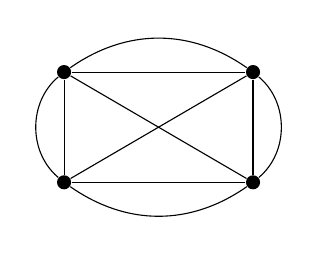
\begin{tikzpicture}[every node/.style={circle,fill,inner sep=1.8pt}]
        \node (A) at (0,1.4) {};
        \node (B) at (2.4,1.4) {};
        \node (C) at (2.4,0) {};
        \node (D) at (0,0) {};
        \draw (A)--(B)--(C)--(D)--(A);
        \draw (A)--(C); \draw (B)--(D);
        \draw (A) to[bend left=35] (B);
        \draw (B) to[bend left=50] (C);
        \draw (C) to[bend left=35] (D);
        \draw (D) to[bend left=50] (A);
    \end{tikzpicture}
    \end{center}
\end{exercise}

\begin{exercise}{10}
    Each of the five platonic solids (tetrahedron, cube, octahedron,
    dodecahedron, icosahedron) has a skeleton graph. For each of these five
    graphs: find a Hamiltonian cycle; determine if it is Eulerian, and if so,
    find an Euler tour.
\end{exercise}

\begin{exercise}{11}
    Let $Q_n$ be the graph whose vertices are all $n$-bit strings, two being
    adjacent iff they differ in exactly one bit.
    \begin{enumerate}[label=(\alph*)]
        \item Draw the cube $Q_3$.
        \item Find a Hamiltonian cycle in $Q_3$.
        \item Describe a method for constructing a Hamiltonian cycle in $Q_n$ for
              each $n$. Think recursively.
        \item Find an Eulerian cycle in $Q_4$.
    \end{enumerate}
\end{exercise}

\begin{exercise}{12}
    Theorem 64 (Euler): \emph{A connected (simple) graph has an Euler tour iff
    every vertex has even degree.} Using Theorem 64 as a black box (don't re-do
    its proof), show that a connected \emph{multigraph} is Eulerian iff every
    vertex has even degree. (Hint: from any multigraph $G$, construct a simple
    graph $H$ such that applying Theorem 64 to $H$ helps.)
\end{exercise}


\newpage
\section{Chapter 12: Graph Theory II}
% CN 12.7 Exercises (p.447--449)

% ======================================================================
\begin{exercise}{1}
    Draw all trees that have six vertices (every tree on six vertices should be
    identical to one in your set, up to relabelling and redrawing).
\end{exercise}

\begin{exercise}{2}
    The \emph{diameter} of a graph is the length of the longest path in it.
    Prove that every tree of diameter $\ge3$ has a vertex $v$ such that
    \[
        2\le\deg(v)\le n-2,
    \]
    where $n$ is the number of vertices.
\end{exercise}

\begin{exercise}{3}
    If a tree has $k$ vertices of degree 3 and all other vertices are leaves, how
    many leaves does it have?
\end{exercise}

\begin{exercise}{4}
    \begin{enumerate}[label=(\alph*)]
        \item Prove that every tree with at least three vertices has a vertex of
              degree at least 2.
        \item Is there a number $N$ such that every tree with at least $N$
              vertices has a vertex of degree at least 3?
    \end{enumerate}
\end{exercise}

\begin{exercise}{5}
    Prove that a graph $G$ is a tree if and only if for every pair $u,v$ of
    vertices, there is a unique path between them in $G$.
\end{exercise}

\begin{exercise}{6}
    Give an upper bound on the average degree of a tree.
\end{exercise}

\begin{exercise}{7}
    How many spanning trees does the following graph have?
    \begin{center}
    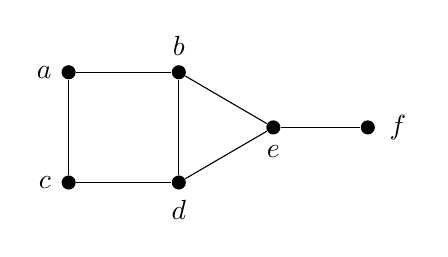
\begin{tikzpicture}[every node/.style={circle,fill,inner sep=1.8pt}]
        \node[label=left:$a$] (a) at (0,1.4) {};
        \node[label=above:$b$] (b) at (1.4,1.4) {};
        \node[label=left:$c$] (c) at (0,0) {};
        \node[label=below:$d$] (d) at (1.4,0) {};
        \node[label=below:$e$] (e) at (2.6,0.7) {};
        \node[label=right:$f$] (f) at (3.8,0.7) {};
        \draw (a)--(b)--(d)--(c)--(a);
        \draw (b)--(e)--(d);
        \draw (e)--(f);
    \end{tikzpicture}
    \end{center}
\end{exercise}

\begin{exercise}{8}
    Apply Kruskal's Greedy Algorithm to find a minimum weight spanning tree in the
    following weighted graph.
    \begin{center}
    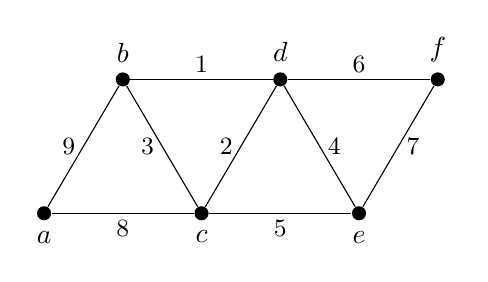
\begin{tikzpicture}[every node/.style={circle,fill,inner sep=1.8pt},
                        lab/.style={fill=none,draw=none,inner sep=1pt,font=\small}]
        \node[label=below:$a$] (a) at (0,0) {};
        \node[label=below:$c$] (c) at (2,0) {};
        \node[label=below:$e$] (e) at (4,0) {};
        \node[label=above:$b$] (b) at (1,1.7) {};
        \node[label=above:$d$] (d) at (3,1.7) {};
        \node[label=above:$f$] (f) at (5,1.7) {};
        \draw (b)--node[lab,above]{1}(d);
        \draw (d)--node[lab,above]{6}(f);
        \draw (a)--node[lab,left]{9}(b);
        \draw (b)--node[lab,left]{3}(c);
        \draw (c)--node[lab,left]{2}(d);
        \draw (d)--node[lab,right]{4}(e);
        \draw (e)--node[lab,right]{7}(f);
        \draw (a)--node[lab,below]{8}(c);
        \draw (c)--node[lab,below]{5}(e);
    \end{tikzpicture}
    \end{center}
\end{exercise}

\begin{exercise}{9}
    Prove that $K_{2,n}$ is planar for all $n$.
\end{exercise}

\begin{exercise}{10}
    Check that Euler's Theorem ($n-m+f=2$) holds for the following graphs:
    \begin{enumerate}[label=(\alph*)]
        \item the cycle $C_n$;
        \item the wheel graph $W_n$, obtained from $C_n$ (the ``rim'') by adding
              a new vertex (the ``hub'') adjacent (via ``spokes'') to every vertex
              of $C_n$;
        \item $K_4$;
        \item the cube $Q_3$ (Exercise 11.11);
        \item the octahedron;
        \item the dodecahedron;
        \item the icosahedron.
    \end{enumerate}
\end{exercise}

\begin{exercise}{11}
    \begin{enumerate}[label=(\alph*)]
        \item Give an upper bound on the average degree of a planar graph.
        \item Give an upper bound on the average degree of a planar graph with no
              triangles.
        \item Give an upper bound on the average degree of a bipartite planar
              graph.
    \end{enumerate}
\end{exercise}

\begin{exercise}{12}
    Prove that every planar graph has a vertex of degree $\le5$.
\end{exercise}

\begin{exercise}{13}
    Let $d\in\N$. A graph is \emph{$d$-regular} if every vertex has degree $d$.
    \begin{enumerate}[label=(\alph*)]
        \item Find the 3-regular planar graph with the fewest vertices.
        \item Find the 3-regular bipartite planar graph with the fewest vertices.
        \item Find the 3-regular nonplanar graph with the fewest vertices.
        \item Describe an infinite family of connected 4-regular planar graphs.
        \item What is the minimum number of vertices of a 5-regular planar graph?
              Can you find such a graph?
        \item Does a 6-regular planar graph exist? Justify your answer.
    \end{enumerate}
\end{exercise}

\end{document}
